\section{Nozioni preliminari}
UDP(Used Datagram Protocol) e TCP(Transmission Control Protocol) sono i protocolli di trasporto(livello 4) più diffusi.
Principali differenze:
\begin{itemize}
    \item TCP è orientato alla connessione, UDP no (vuol dire che non è necessario stabilire una connessione prima di inviare i dati, cosa invece necessaria con TCP)
    \item TCP è un protocollo di trasporto affidabile, UDP è non affidabile(quindi TCP garantisce che i dati arrivino a destinazione e nell'ordine corretto, mentre UDP non lo fa)
\end{itemize}

I pacchetti(PDU) TCP sono chiamati segmenti, mentre i pacchetti UDP sono chiamati datagrammi.

\paragraph{Funzioni principali UDP}
Svolge l'unico compito di incapsulare i dati dell'applicazione in un pacchetto UDP, aggiungendo le informazioni necessarie per la consegna(Multiplexing). Non fornisce alcuna garanzia di consegna o ordine dei pacchetti.
\paragraph{Funzioni principali TCP}
\begin{multicols}{2}
\begin{itemize}
    \item Controllo flusso end to end
    \item Controllo congestione end to end
    \item Ritrasmette le PDU perse o corrotte
    \item Riordina i segmenti ricevuti in ordine corretto
\end{itemize}
\end{multicols}
Il TCP numera i singoli byte che arrivano dal livello applicativo, e non i segmenti; è fondamentale poichè dal livello 3(IP) non arrivano i byte in ordine, ma i pacchetti possono arrivare in ordine sparso.

\subsection{Sock e ports}
Dei concetti fondamentali per il funzionamento di TCP e UDP sono i socket e le porte.
\begin{itemize}
    \item Socket: è un punto finale di una connessione di rete, rappresentato da:
    \begin{itemize}
        \item Indirizzo IP: identifica un host sulla rete
        \item Porta: identifica un'applicazione in esecuzione su quell'host 
    \end{itemize}
    I socket sono utilizzati per inviare e ricevere dati tra applicazioni su host diversi.
    \item Porta: è un numero che identifica un'applicazione in esecuzione su un host. Le porte sono numerate da 0 a 65535 e sono suddivise in tre categorie: well-known ports, registered ports e dynamic/private ports.
\end{itemize}
Il numero di porta è un numero a 16 bit che identifica un'applicazione in esecuzione su un host. Quando un client invia una richiesta HTTP a un server web, utilizza la porta 80 per comunicare con il server. Il server ascolta sulla porta 80 e risponde alla richiesta del client.

\begin{figure}[h!]
    \centering
    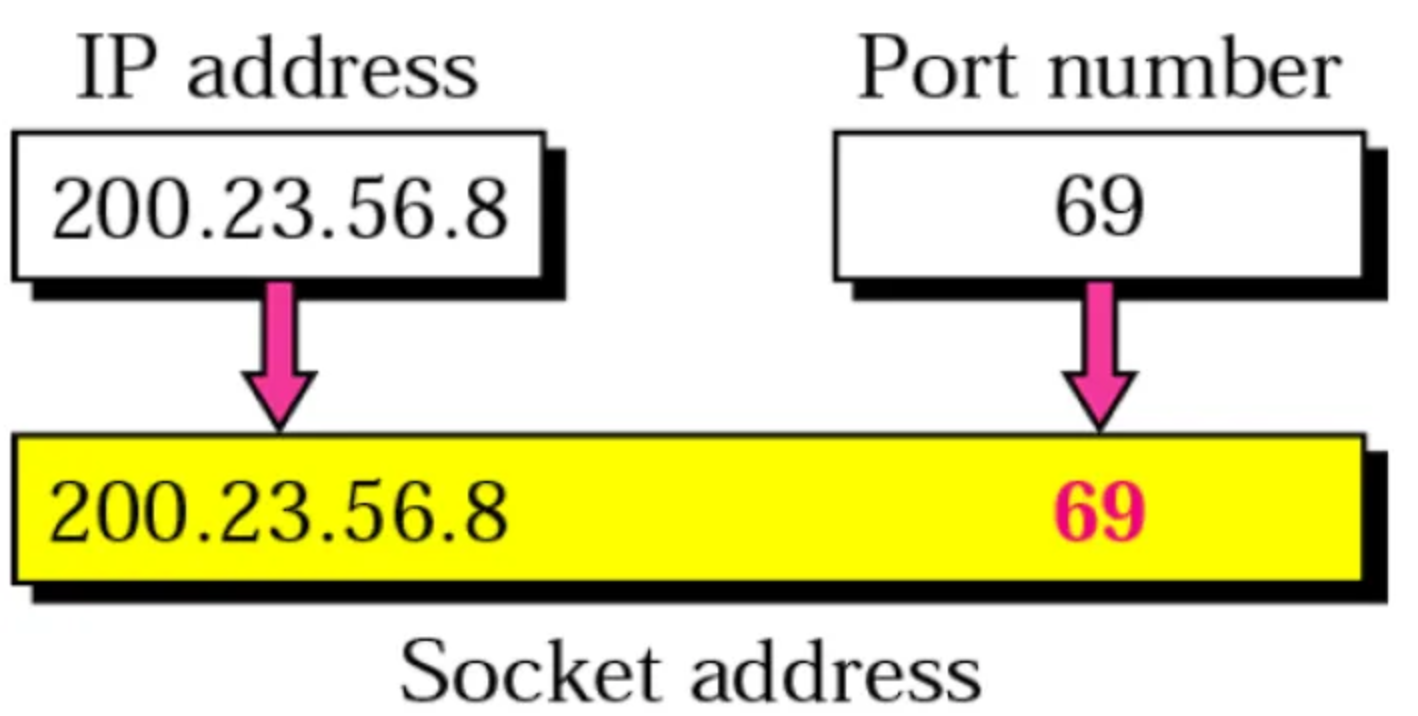
\includegraphics[width=0.6\textwidth]{images/socket_port.png}
    \caption{Relazione tra socket, indirizzo IP e porta}
    \label{fig:socket_port}
\end{figure}

Le porte sono numerate da 0 a 65535 e sono suddivise in tre categorie:
\begin{itemize}
    \item Well-known ports: da 0 a 1023, utilizzate da applicazioni di sistema e protocolli standard (es. HTTP su porta 80, HTTPS su porta 443, DNS(traduce il nome "simbolico" del servizio web per il web server) su porta 53)
    \item Registered ports: da 1024 a 49151, utilizzate da applicazioni registrate presso l'IANA
    \item Dynamic/Private ports: da 49152 a 65535, utilizzate per connessioni temporanee e dinamiche
\end{itemize}

Tramite i numeri di porta è possibile identificare a livello 4 con quale applicazione sto inviando/ricevendo dati

Come identificare un flusso dati in internet?

\begin{figure}[h!]
    \centering
    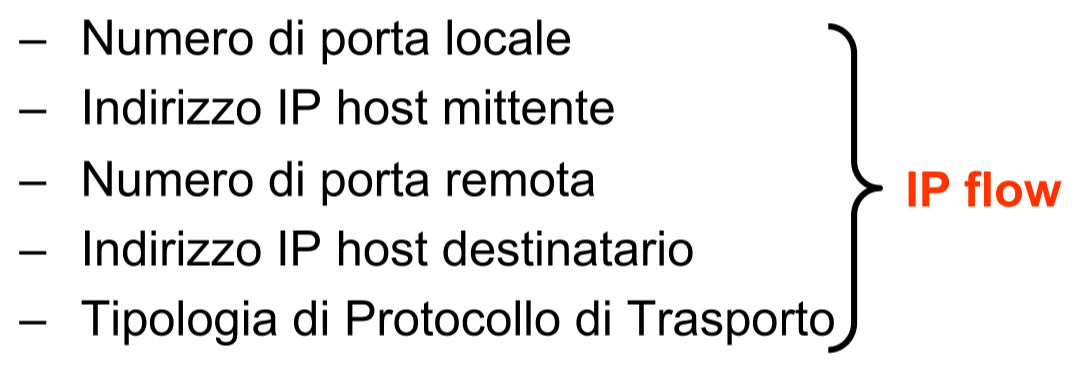
\includegraphics[width=0.5\textwidth]{images/flusso_IP.png}
    \caption{Identificazione di un flusso dati tramite indirizzi IP e numeri di porta (tuple a 4 campi)}
    \label{fig:flussoIP}
\end{figure}

\begin{figure}[h!]
    \centering
    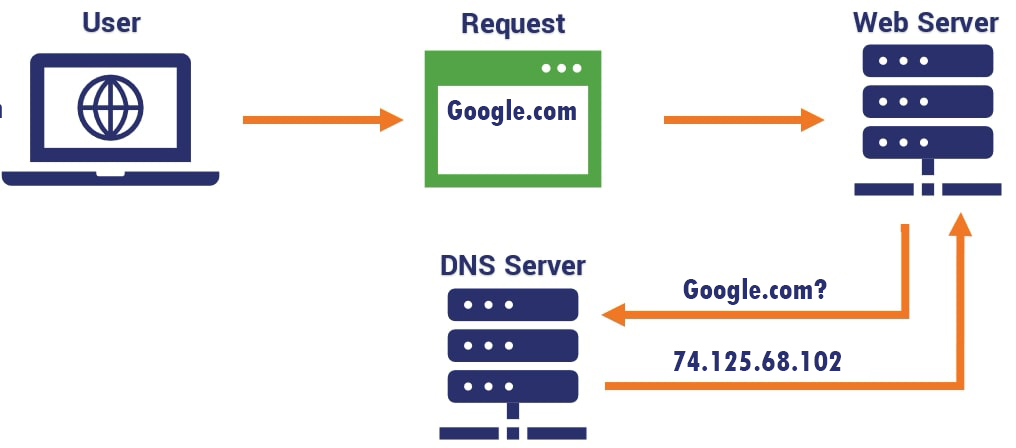
\includegraphics[width=0.5\textwidth]{images/DNS.jpg}
    \caption{Esempio di funzionamento del DNS: risoluzione di un nome simbolico in indirizzo IP, tramite DNS server}
    \label{fig:dns_example}
\end{figure}
traduce nomi comprensibili come www.amazon.com in indirizzi IP utilizzati dai computer, ad esempio 192.0.2.44
\newpage
\section{UDP - datagram}

è il più veloce del TCP poichè non esegue molte funzioni come l'ordinamento dei pacchetti 
i pacchetti sono da 32 bit, ossia 4 byte:
\begin{itemize}
    \item datagram: 16 bit
    \item pseudoheader: 16 bit
\end{itemize}

Si occupa di fare multiplexing(trasmissione) e demultiplexing(ricezione) dei dati, ovvero incapsula i dati dell'applicazione in un pacchetto UDP e aggiunge le informazioni necessarie per la consegna.
Viene usato soprattutto per applicazioni in tempo reale, come servizi streaming live.

\paragraph{Struttura del datagram UDP}

\begin{figure}[h!]
    \centering
    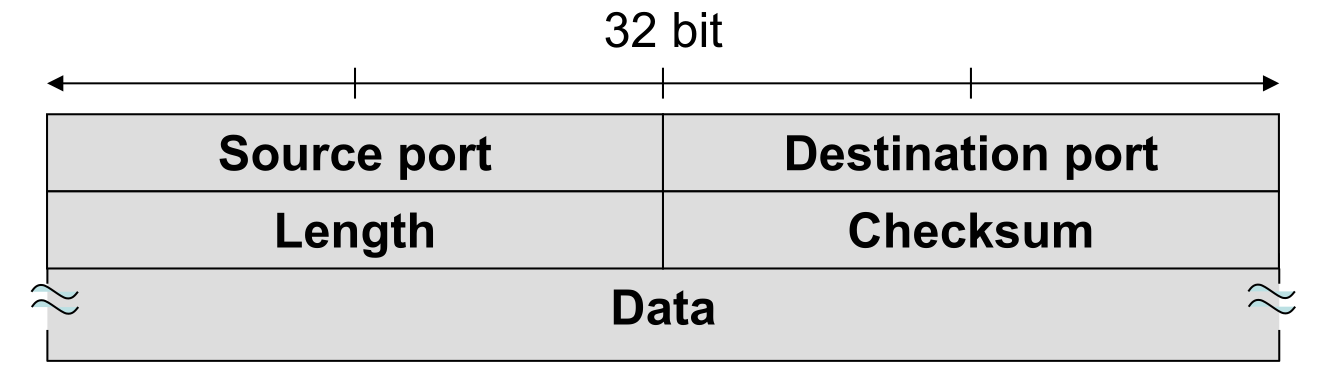
\includegraphics[width=0.7\textwidth]{images/datagram_udp.png}
    \caption{Struttura del datagram UDP}
    \label{fig:datagramudp}
\end{figure}

\begin{itemize}
    \item Source port e destination port(indirizzo IP del mittente/destinatario): 16 bit ciascuno
    \item Length (dimensione del datagram): 16 bit, quindi può rappresentare valori da 0 a $2^{16}-1 = 65535$ bytes, ma il campo include anche l'header, quindi la dimensione massima di un datagram UDP è 65535 byte.
    \item Checksum: 16 bit, utilizzato per verificare l'integrità dei dati del datagram. Il checksum è calcolato su un pseudoheader che include informazioni sull'indirizzo IP del mittente e del destinatario, oltre alla lunghezza del datagram e al protocollo utilizzato (UDP in questo caso). Il pseudoheader non viene trasmesso, ma viene utilizzato solo per il calcolo del checksum. 
    \item Data: dimensione variabile, contiene i dati dell'applicazione
\end{itemize}


\begin{figure}[h!]
    \centering
    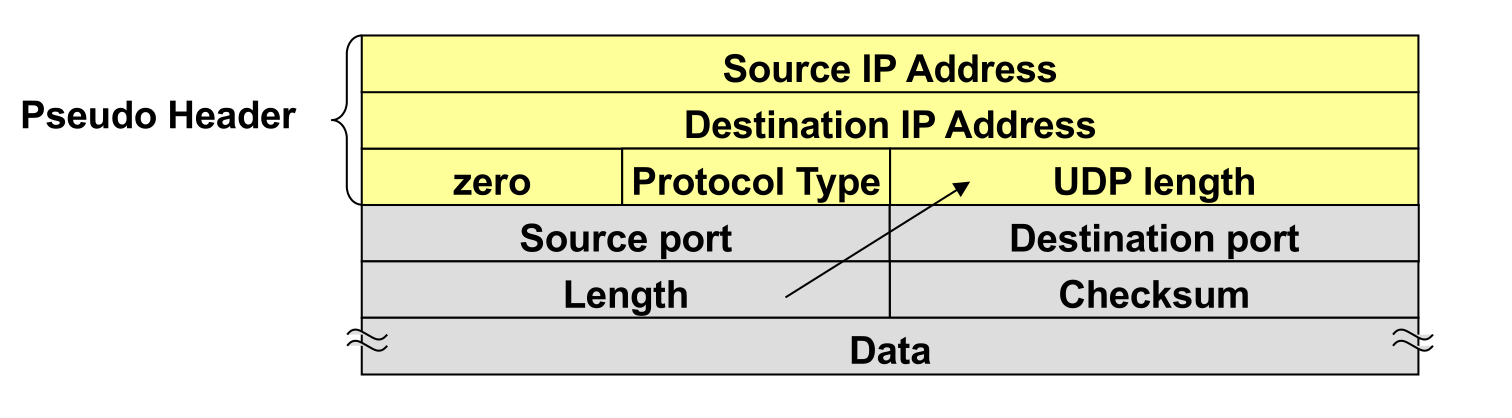
\includegraphics[width=0.7\textwidth]{images/pseudoheaderUDP.png}
    \caption{Pseudoheader UDP utilizzato per il calcolo del checksum}
    \label{fig:psudoheaderudp}
\end{figure}

Nello pseudoheader sono presenti informazioni come il campo Protocol Type viene preso direttamente dal livello 3(protocollo IP).

Il checksum è la somma di controllo, è una tecnica di verifica veloce di controllo errore, non è affidabile al 100\%, è comunque ottimo perchè è veloce  
\begin{itemize}
    \item Se il checksum è 0, significa che non ci sono errori, non affidabile.
    \item Se il checksum è diverso da 0, significa che ci sono errori, sicuramente(condizione necessaria).
\end{itemize}
\subsection{Calcolo checksum}
Il valore del checksum prima della trasmissione è impostato a 0.
 \paragraph{In trasmissione}
In tramissione vengono sommate in binario tutte le righe(mezze righe da 16 bit) del datagram, faccio il complemento ad 1(NOT) di questo risultato. Questo è il checksum inviato nel datagram di trasmissione.
\paragraph{In ricezione}
In ricezione viene ricevuto il datagram, con all'interno il checksum calcolato precedentemente in trasmissione. 

Viene calcolato nuovamente il checksum del datagram ricevuto, sommando in binario tutte le righe(mezze righe da 16 bit) del datagram, e sommandolo al checksum ricevuto. 

Se il risultato è diverso da 0 significa che i due valori calcolati in ricezione e trasmissione sono differenti, perciò c'è un errore.


\begin{figure}[h!]
    \centering
    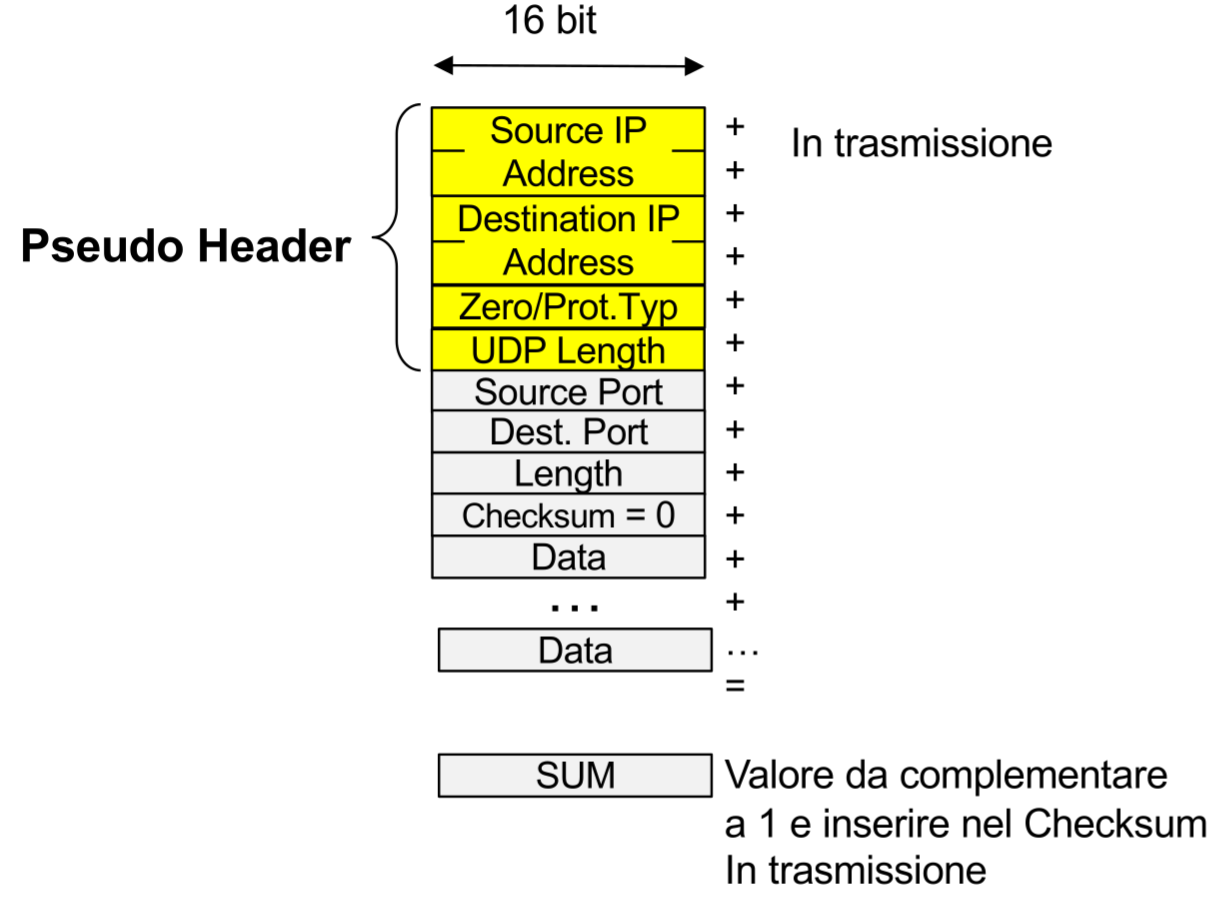
\includegraphics[width=1\textwidth]{images/checksum_udp.png}
    \caption{Esempio di calcolo del checksum UDP}
    \label{fig:checksumudp}
\end{figure}

\newpage
\section{TCP - segmento}
Nei processi TCP viene utilizzata una coppia di socket per identificare un flusso di dati. Ogni socket è identificato da una tupla a 4 campi:
\begin{multicols}{2}
\begin{itemize}
    \item Indirizzo IP del mittente
    \item Porta del mittente
    \item Indirizzo IP del destinatario
    \item Porta del destinatario
\end{itemize}
\end{multicols}

La connessione è full duplex $\rightarrow$ comunicazione affidabile, se qualcosa va storto chiede la ritrasmissione del pacchetto errato.

Il tcp è un protocollo greedy, ingordo, tende a prendere tutta la banda di cui necessita; questo protocollo non evita le congestioni ma le provoca, però quando le provoca cerca di risolverle.

L'affidabilitò di TCP sta nei riscontri cumulativi che gli permettono di gestire le seguenti problematiche:
\begin{itemize}
    \item Controllo di congestione e2e: regolazione del rate di trasmissione così da utilizzare completamente la banda disponibile evitando che la rete collassi
    \item Controllo del flusso e2e: regolarizza il rate di trasmissione per evitare la saturazione del buffer di ricezione
\end{itemize}

\begin{figure}[h!]
    \centering
    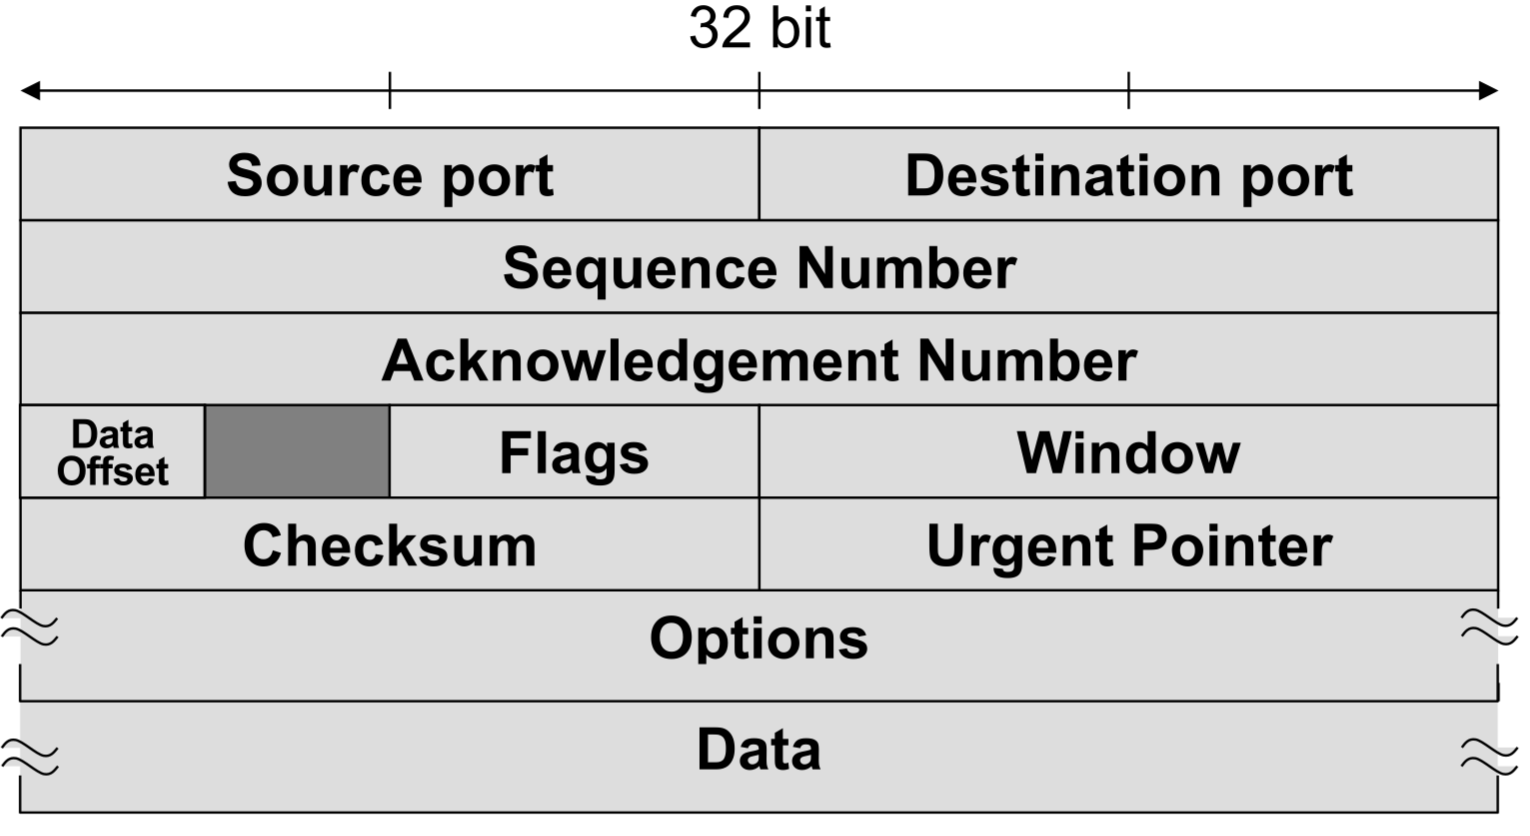
\includegraphics[width=0.8\textwidth]{images/segmento_tcp.png}
    \caption{Struttura del segmento TCP}
    \label{fig:segmentotcp}
\end{figure}

I pacchetti in tcp vengono chiamati segmenti, così strutturati:
\begin{itemize}
    \item source port/destination port: 16 bit ciascuna e identificano il mittente e il destinatario del segmento
    \item sequence number: 32 bit, numero di sequenza del primo byte del segmento, utilizzato per ordinare i segmenti ricevuti ; i byte del livello applicativo (che costituiranno il payload dei
diversi segmenti trasmessi) sono numerati in modo continuo partendo da un valore casuale(zero relativo). 

Nel campo Seq. Number si inserisce poi il numero di sequenza (di questa numerazione continua)
relativo al primo byte contenuto nel campo Data
\begin{figure}[h!]
    \centering
    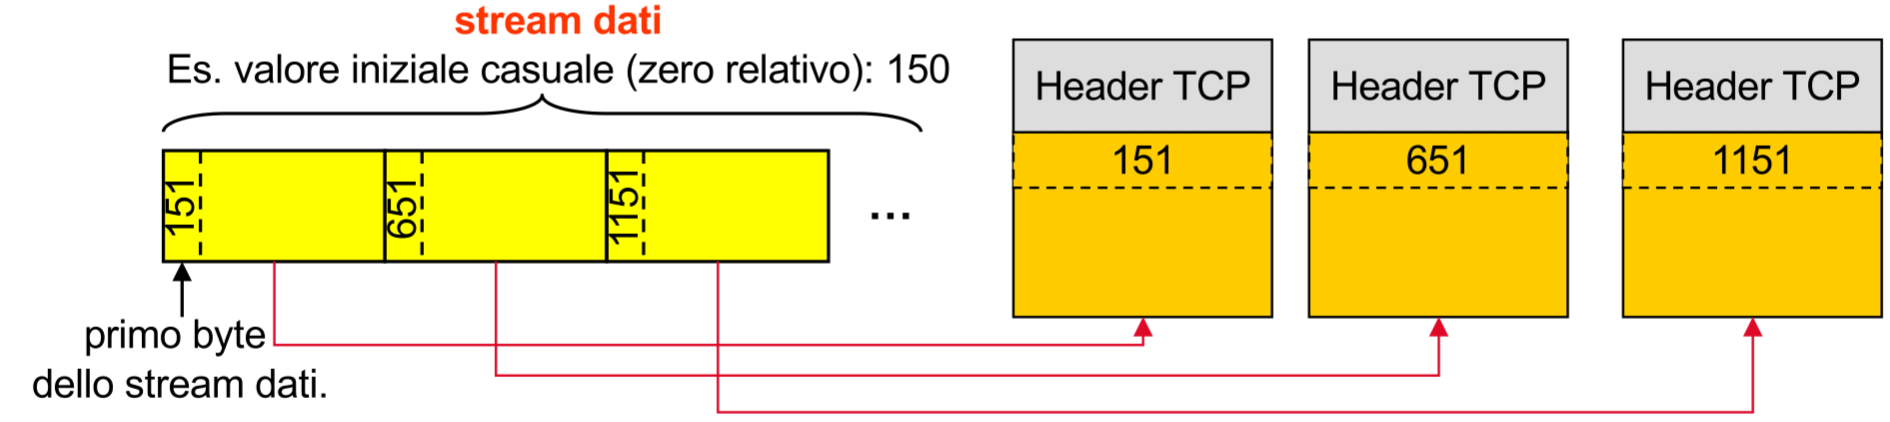
\includegraphics[width=0.9\textwidth]{images/sequence_number.png}
    \caption{Esempio di utilizzo del campo Sequence Number nei segmenti TCP}
    \label{fig:sequencenumber}
\end{figure}
    \item ackwoledgment number: 32 bit, nel campo ack.number si inserisce il numero di sequenza del primo byte che ci si aspetta di ricevere (quindi il numero di sequenza del primo byte che non è stato ricevuto), si usa per capire fino a che punto il segmento è stato ricevuto correttamente. Così facendo so anche da che punto riprendere la trasmissione dei dati.(è utile a dare un riscontro di ciò che mi sta inviando il mittente, tenendolo aggiornato sulla correttezza di ciò che mi ha inviato, connessione full duplex appunto); può essere anche un campo vuoto, 0.
    \item data offset: 4 bit, indica la lunghezza dell'header del TCP
    \item flags: 6 bit, sono dei flag di controllo che indicano lo stato della connessione TCP:
    \begin{itemize}
        \item URG: indica se il segmento contiene dati urgenti.
        \item ACK: acknowledgment number
        \item PSH: push, richiesta di invio immediato dei dati al livello applicativo
        \item RST, SYN, FIN: reset, synchronize, finish della connessione 
        \end{itemize}
    \item window: è un campo utilizzato nella gestione del controllo di flusso, indica la dimensione della finestra di ricezione, ovvero la quantità di dati che il mittente può inviare prima di ricevere un acknowledgment dal destinatario. La dimensione della finestra può variare durante la connessione in base alla disponibilità di buffer del destinatario.
    \item urgent pointer: indica i dati che il ricevitore deve elaborare per prima
    \item checksum: è come in UDP
    \item options: almeno 32 bit, è opzionale, può contenere info di configurazione del segmento TCP 
\end{itemize}


\subsection{Apertura connessione client-server (3way handshake)}
 
\begin{figure}[h!]
    \centering
    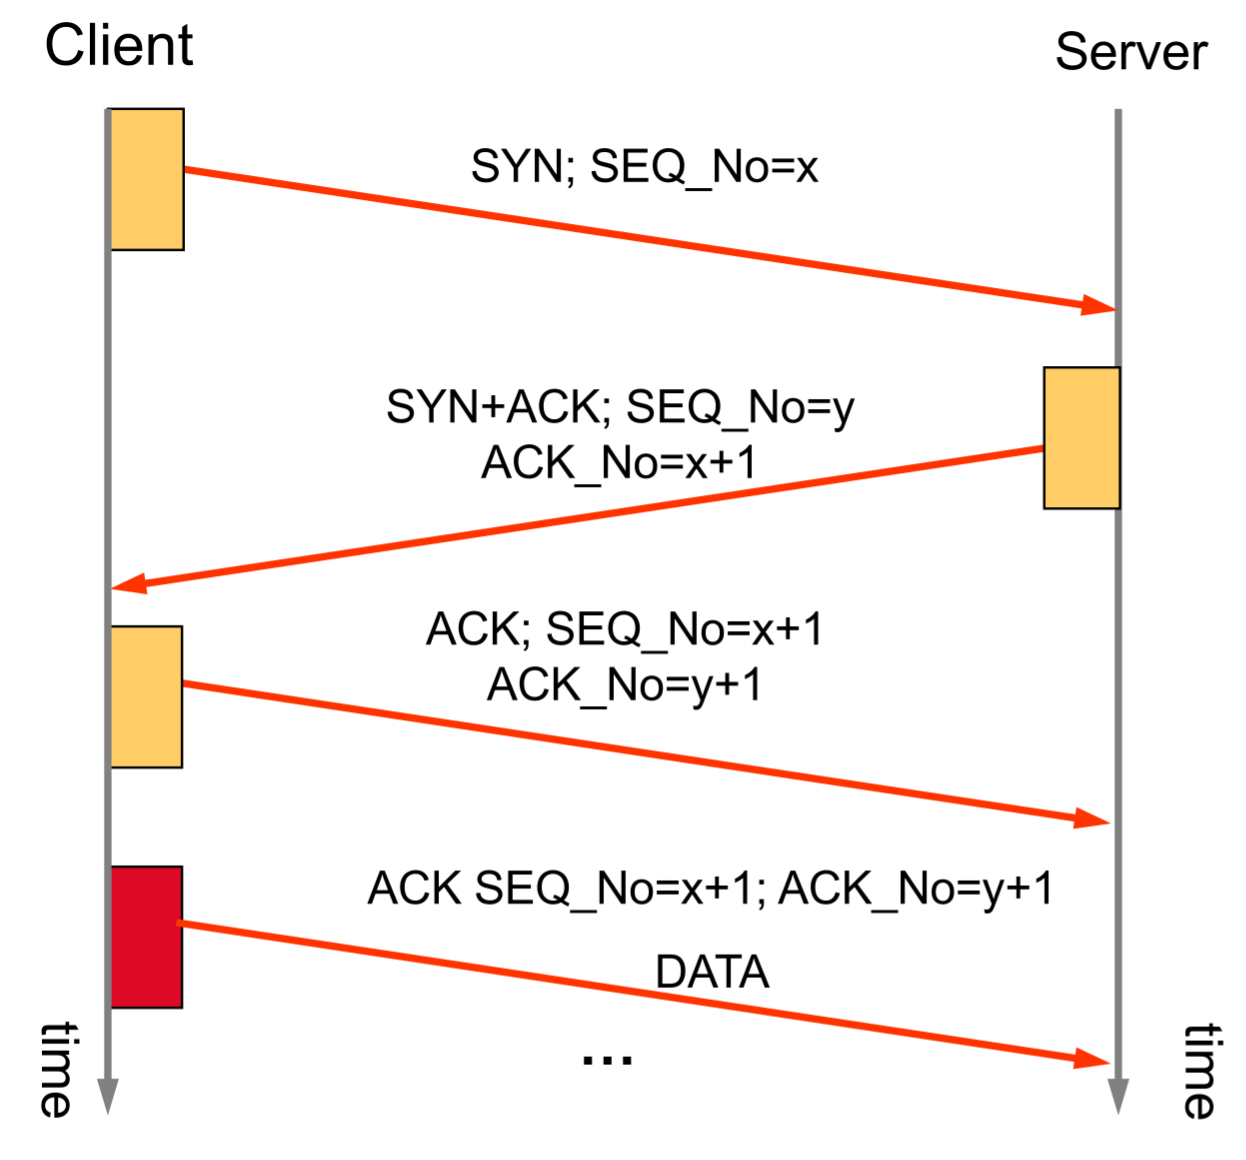
\includegraphics[width=0.7\textwidth]{images/three_w_hs1.png}
    \caption{Three-way handshake: stabilimento della connessione TCP tra client e server}
    \label{fig:threewayhandshake}
\end{figure}

La connessione viene sempre aperta dal client.

Quando ricevo un segmento ho bisogno di sapere in che modo sta contando i byte il mittente; 

Il client sceglie lo zero relativo, ossia il numero di sequenza(sequence number scelto casualmente, $SEQ.NUMBER = x$) da cui partire per numerare i byte che invierà al server, inviando un segmento vuoto in cui setta il flag $SYN = 1$,($ACK = 0$ all'inizio della comunicazione) così da iniziare la comunicazione.

A questo punto il server risponde alla richiesta del client, inviando:
\begin{itemize}
    \item un segmento vuoto con $SYN = 1$ e $ACK = 1$(questo flag a 1 fa capire al client che il campo ACKNUMBER è stato modificato), in cui il numero di sequenza è $SEQ.NUMBER = y$(per i dati che il server invierà, non dimenticare che la comunicazione è full duplex) e il numero di ack è $ACK.NUMBER = x + 1$ (il server ha ricevuto la richiesta del client, quindi il numero di ack è incrementato di 1)
    \item un segmento con i dati richiesti dal client, in cui il numero di sequenza è $SEQ.NUMBER = y + 1$ e il numero di ack è $ACK.NUMBER = x + 1$
\end{itemize}

 

Per terminare la "conversazione" il client invia un segmento(vuoto, ossia senza dati) con il flag SYN a 0, e conferma la corretta ricezione del messaggio precedente (y) con l'ACK.NUMBER ricevuto dal server più di 1(y + 1).

Quello in rosso nell'immagine è un ulteriore segmento, uguale al precedente, ma "pieno", ossia con i dati da inviare.

\subsection{Chiusura connessione}
La chiusura della connessione puà essere avviata da uno dei due host, il client o il server(tipicamente la chiude il client).

\begin{figure}[h!]
    \centering
    \begin{minipage}{0.48\textwidth}
        \centering
        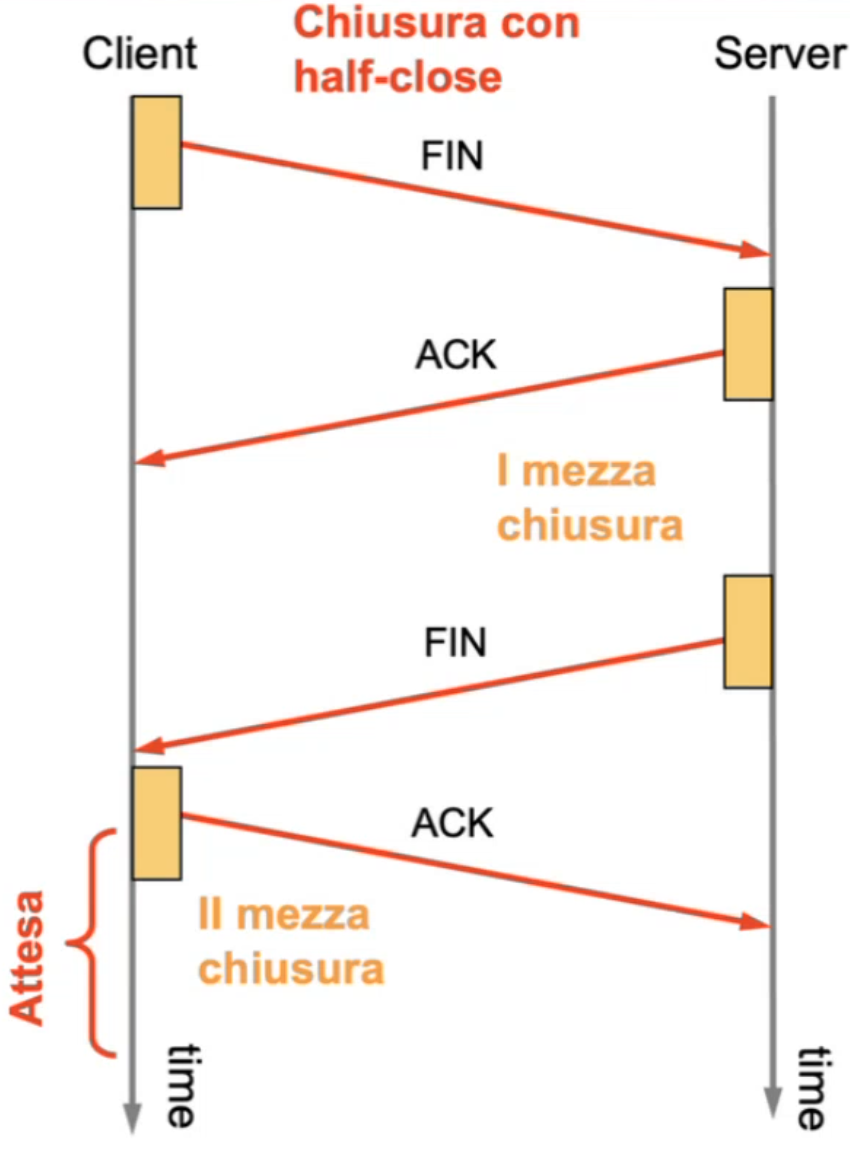
\includegraphics[width=\textwidth]{images/halfclosetcp.png}
        \caption{Chiusura della connessione TCP tramite half-close}
        \label{fig:halfclosetcp}
    \end{minipage}\hfill
    \begin{minipage}{0.48\textwidth}
        \centering
        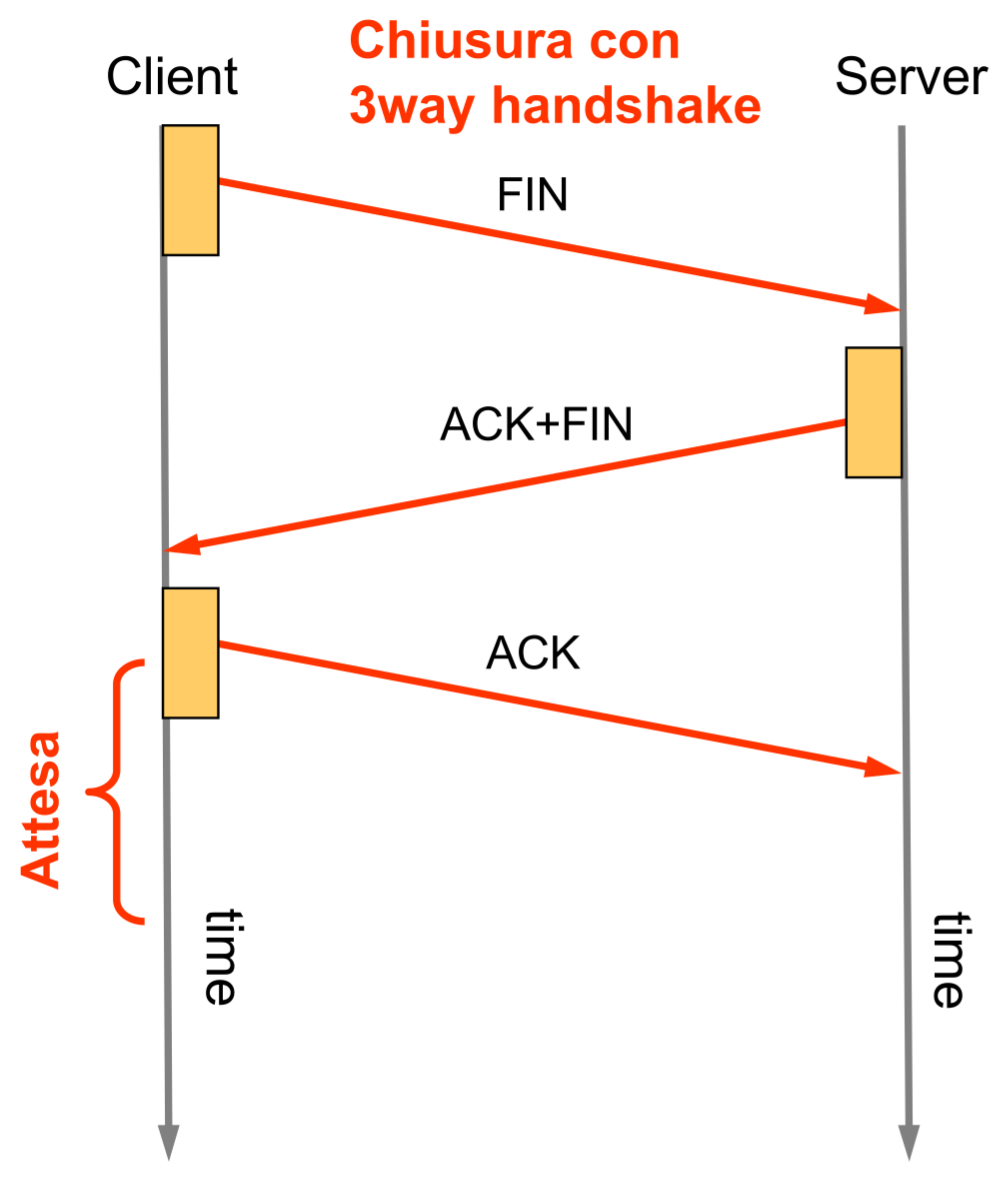
\includegraphics[width=\textwidth]{images/3wayclose.png}
        \caption{Chiusura della connessione TCP tramite 3-way handshake}
        \label{fig:3wayclose}
    \end{minipage}
\end{figure}

\paragraph{Chiusura con half-close}
La chiusura della connessione avviene tramite due mezze chiusure:
\begin{itemize}
    \item prima mezza chiusura:
    \begin{itemize}
            \item Il client invia un segmento con il flag FIN a 1, per indicare che non invierà più dati al server.(inizio I mezza chiusura) 
            \item Il server continua ad inviare i dati finchè non termina e invia un segmento con flag FIN settato.(fine I mezza chiusura)
    \end{itemize}
    \item seconda mezza chiusura:
    \begin{itemize}
            \item Il server invia un segmento con il flag FIN a 1 e il flag ACK a 1, per indicare che non invierà più dati al client.(inizio II mezza chiusura) 
            \item Il client risponde con un segmento con il flag ACK a 1, per confermare la ricezione della richiesta di chiusura del server. (fine II mezza chiusura)
    \end{itemize}
\end{itemize} 


\newpage
\paragraph{Chiusura con 3way handshake}

in risposta al segmento FIN inviato
dal client, il server invia un unico segmento con
FIN+ACK settati (e con eventualmente gli ultimi
dati).

Questa soluzione non prevede che il server invii
ulteriori dati e il client risponde con il segmento di ACK di
chiusura della connessione.



\paragraph{TIMEWAIT}
in entrambe le tecniche (con
half-close o 3way handshake) dopo il segmento
di ACK si avvia un timer (Time Wait) prima della
definitiva chiusura della connessione. Può
succedere, infatti, che il segmento ACK vada
perso e il server ritrasmetta il suo FIN. Il client
deve quindi essere ancora in grado di poter
ritrasmettere l'ACK finale.
\newpage
\subsection{TCP sequenze di stati}
\subsubsection{TCP client}
\begin{figure}[h!]
    \centering
    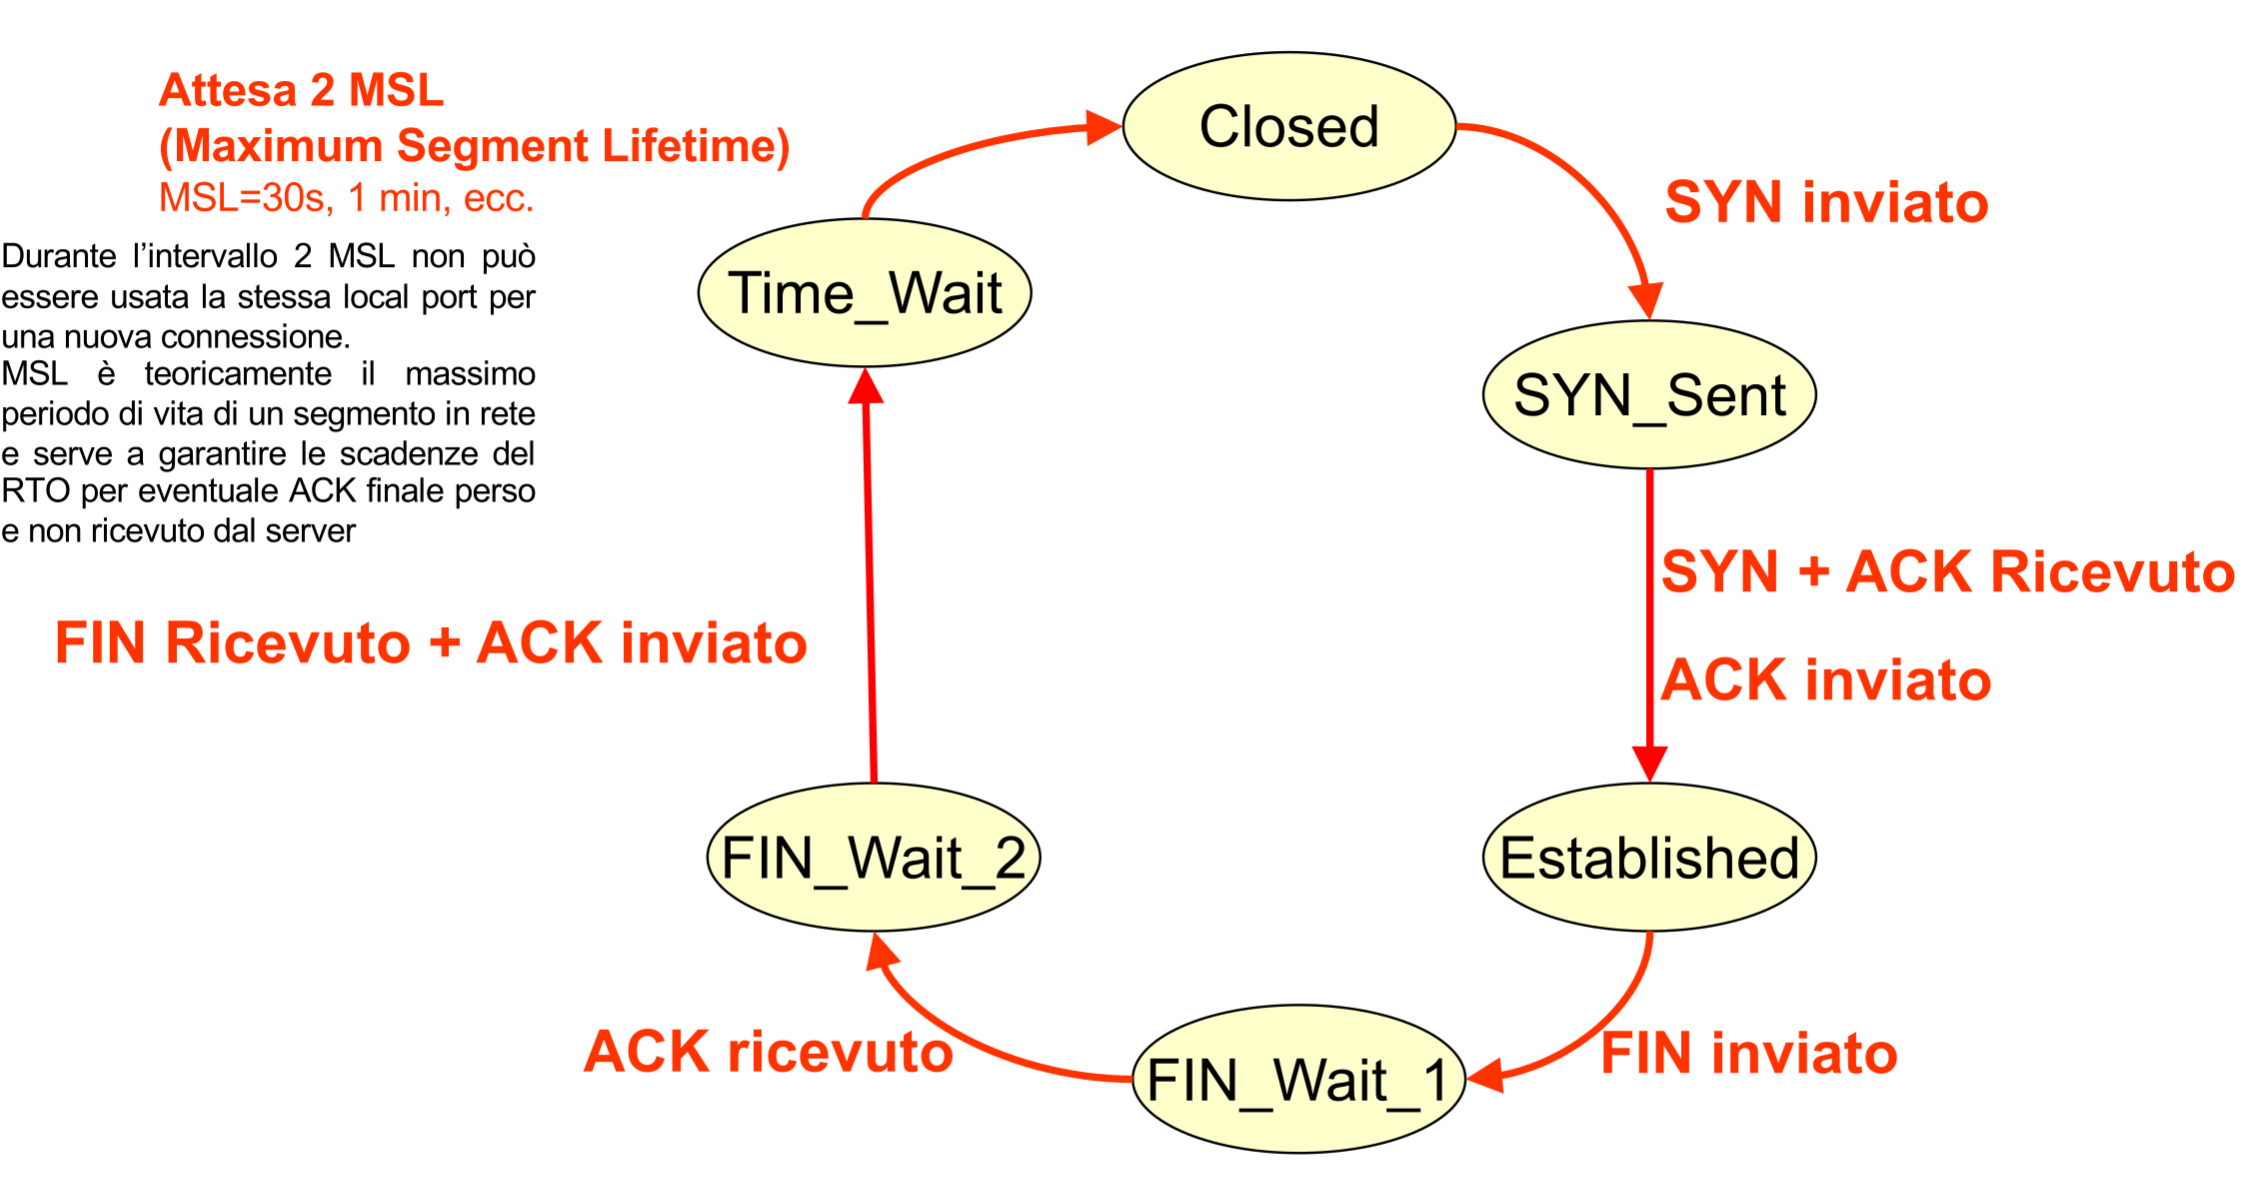
\includegraphics[width=1.1\textwidth]{images/tcpstaticlient.png}
    \caption{Sequenza di stati TCP lato client}
    \label{fig:tcpstaticlient}
\end{figure}
\subsubsection{TCP server}

\begin{figure}[h!]
    \centering
    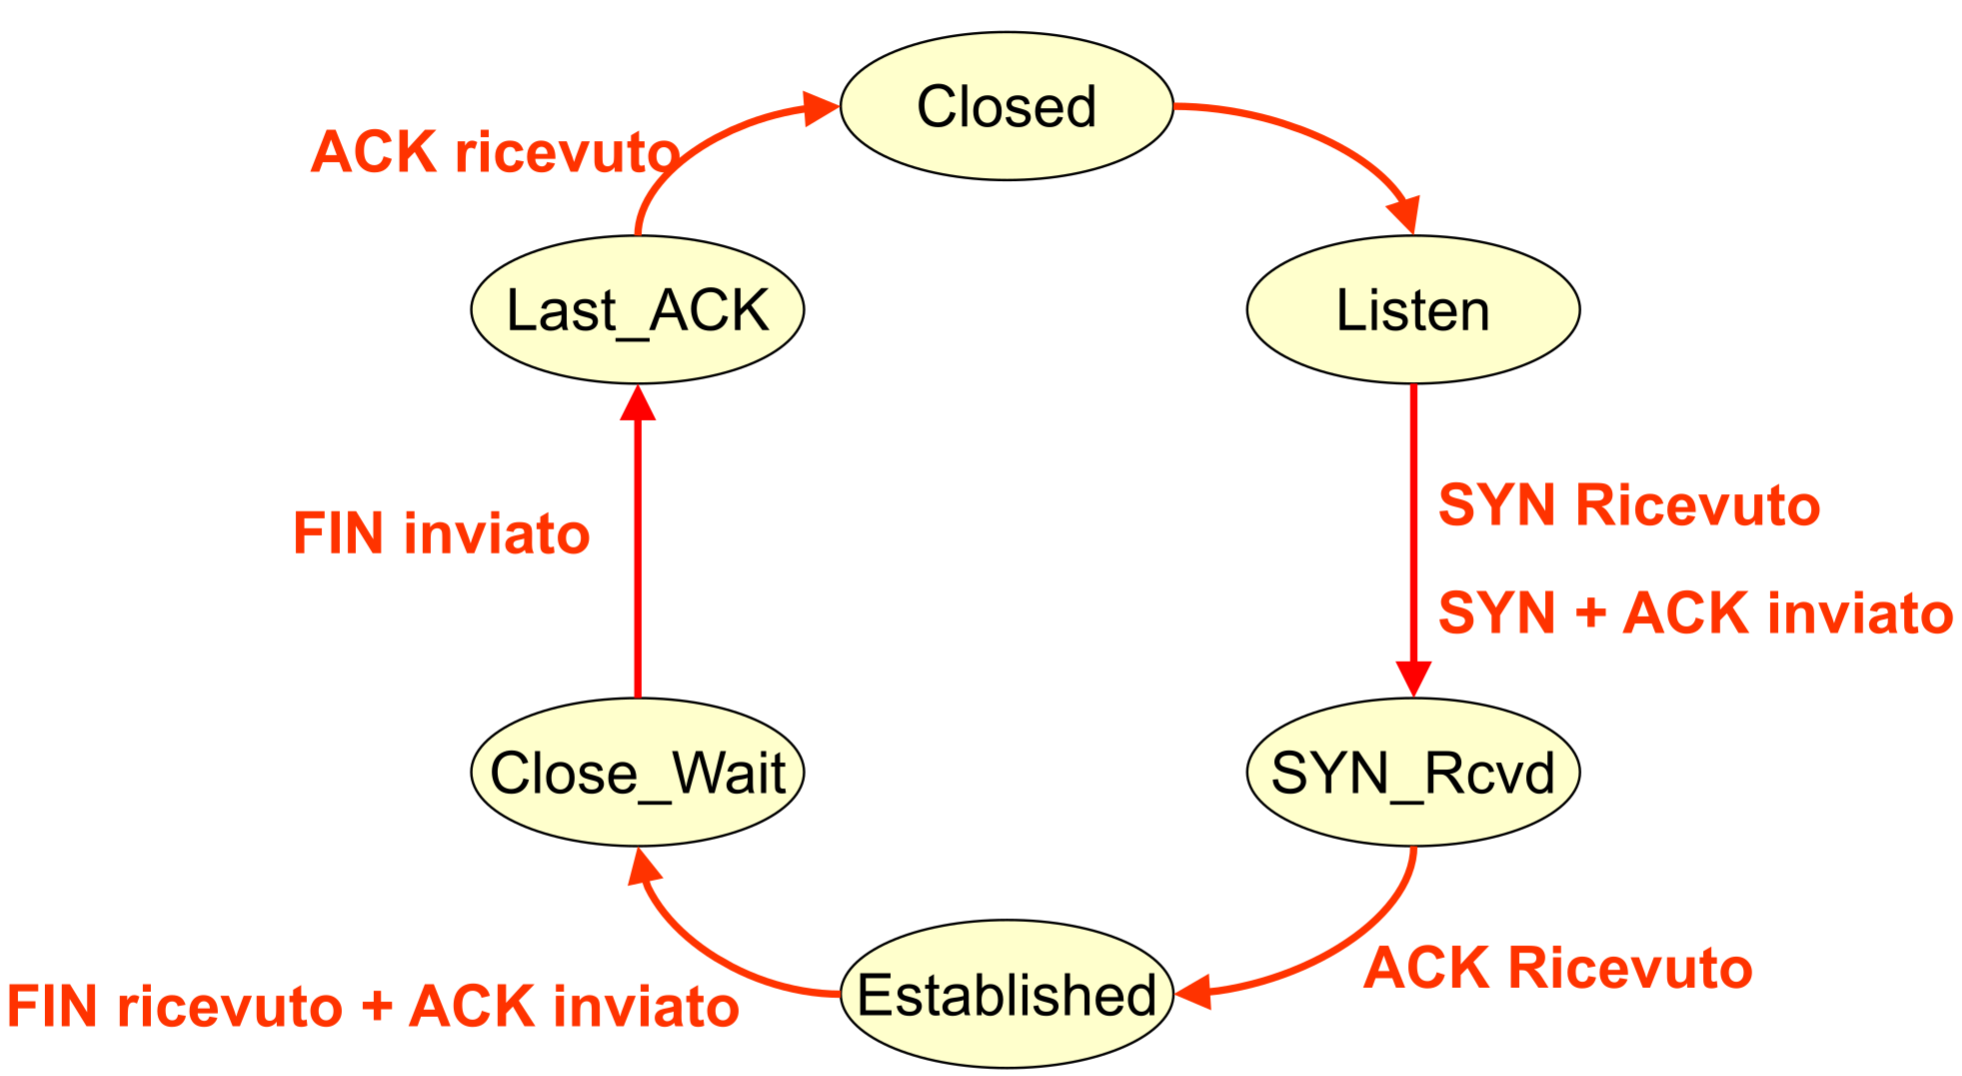
\includegraphics[width=1\textwidth]{images/tcpstatiserver.png}
    \caption{Sequenza di stati TCP lato server}
    \label{fig:tcpstateserver}
    \end{figure}
\newpage

\subsection{Trasmissione dei segmenti - sliding window}
Il TCP usa un meccanismo di trasmissione dei segmenti basato su finestre scorrevoli, finestra di trasmissione e finestra di ricezione; in base alla loro larghezzo si possono inviare più o meno bytes.

Attua "self-clocking", ossia il mittente regola la velocità di invio dei segmenti in base alla velocità di ricezione del destinatario. Non c'è una velocità fissa delle sliding windows.

 \subsubsection{Round trip time - RTT}
Quando invia un segmento, il mittente deve attendere un certo tempo prima di ricevere un (riscontro)acknowledgment dal destinatario. Questo tempo è chiamato round trip time (RTT) e rappresenta il tempo necessario per inviare un segmento e ricevere l'ACK.
 
Data W, dimensione della finestra di trasmissione, e RTT, il tempo di round trip, la velocità media di trasmissione dei segmenti è data da:

\begin{equation}
    \text{rate medio} = \frac{W}{RTT}
\end{equation}

Come miglioro questo rate? 

Si può agire solo sulla dimensione della finestra W, non sul RTT.

\begin{figure}[h!]
    \centering
    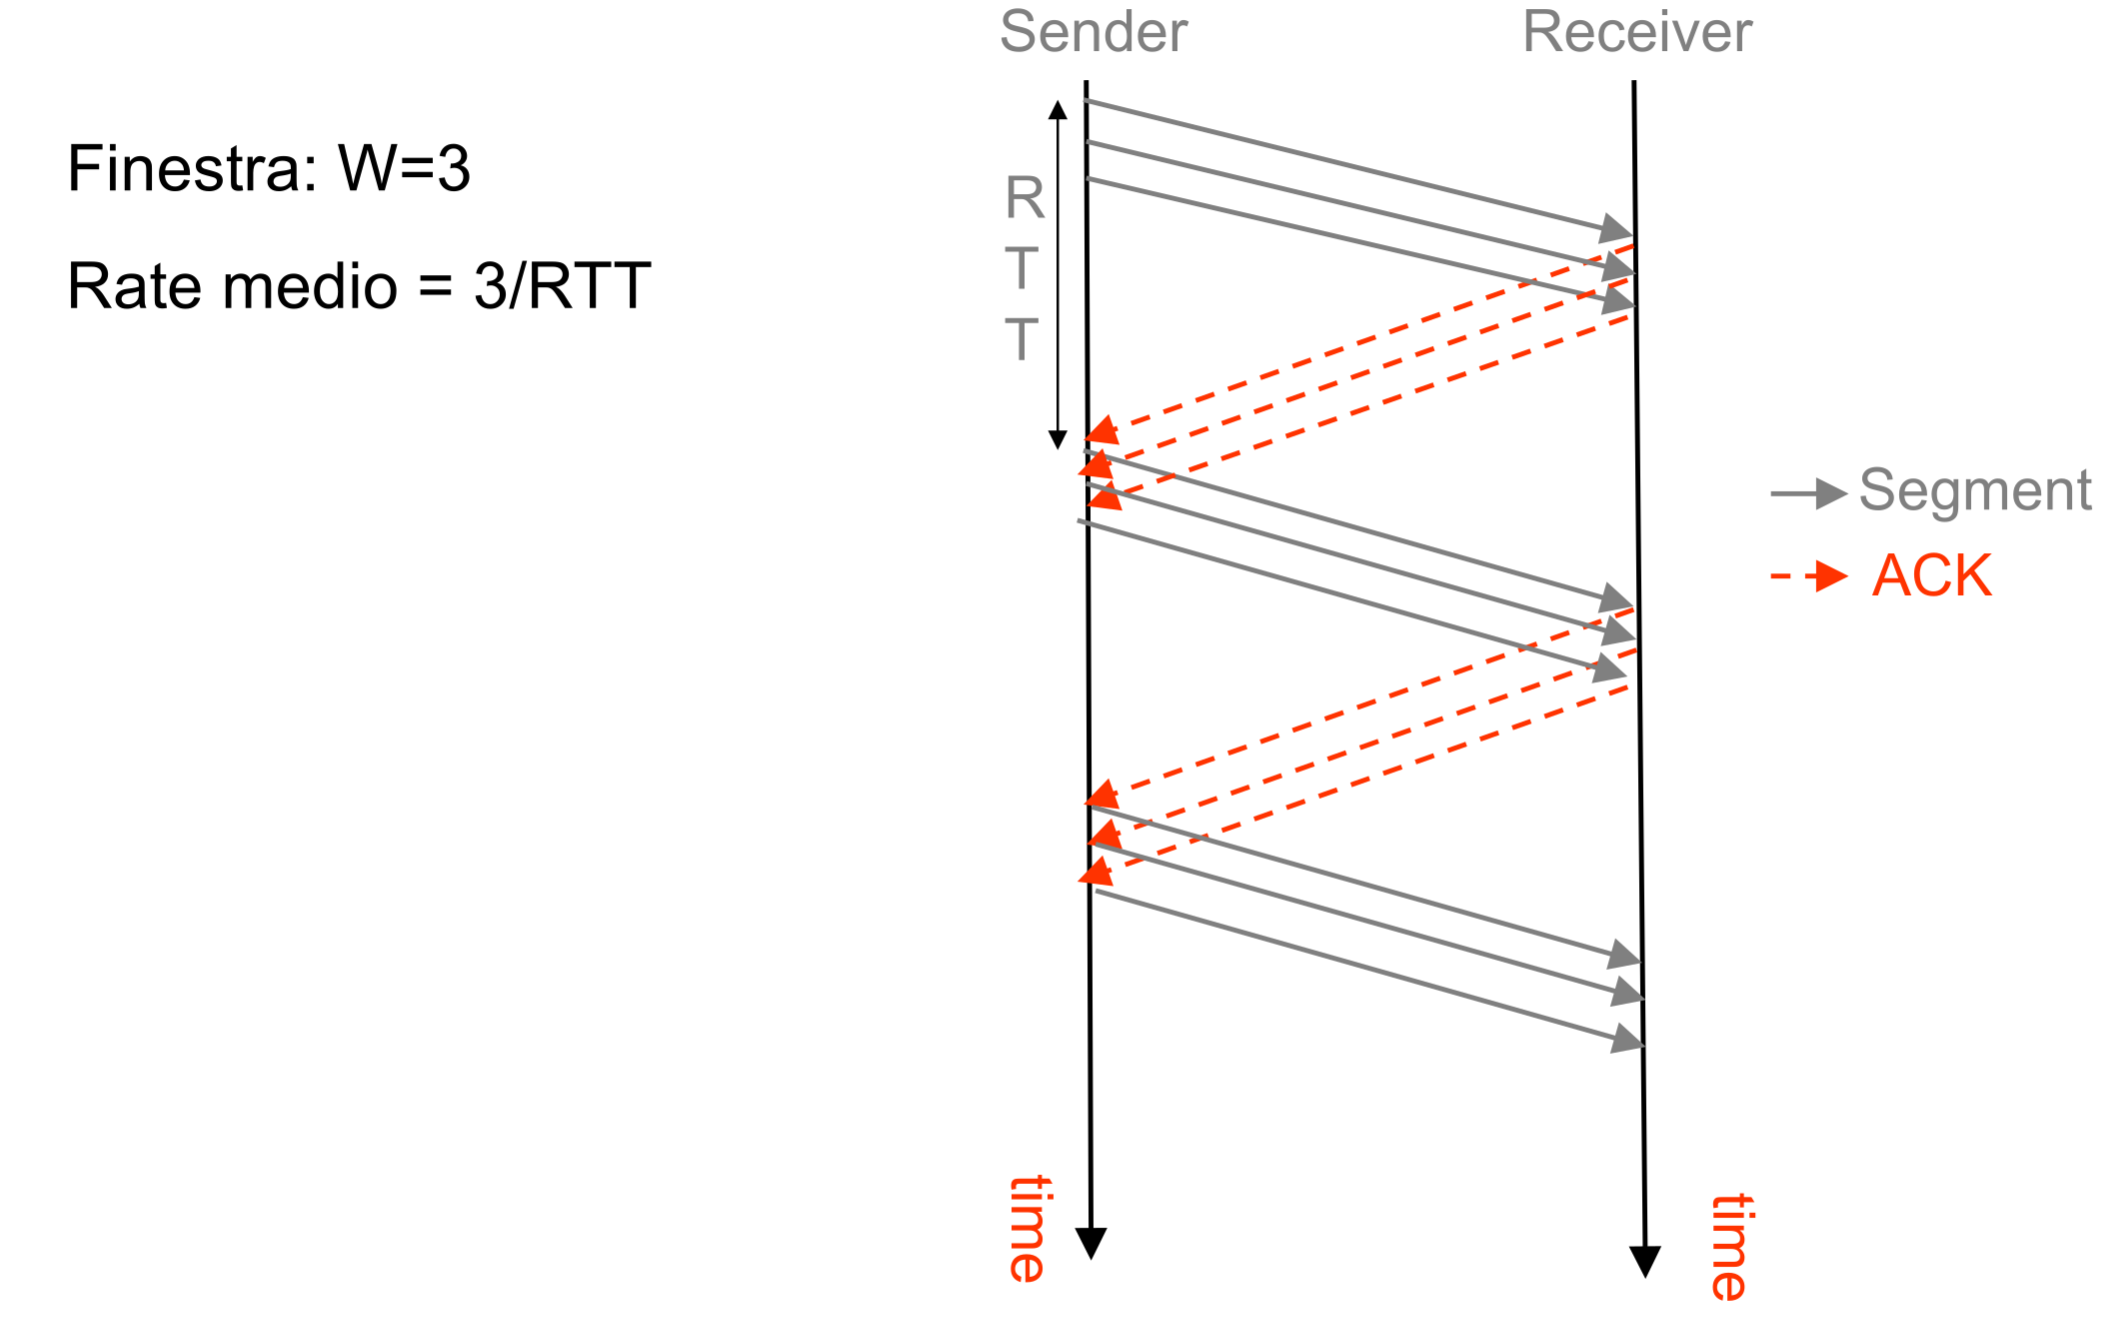
\includegraphics[width=1\textwidth]{images/rttsliding.png}
    \caption{Esempio di sliding window e round trip time (RTT)}
    \label{fig:rttsliding}
\end{figure}
\newpage

\subsection{Finestre di trasmissione e ricezione}
\begin{figure}[h!]
    \centering
    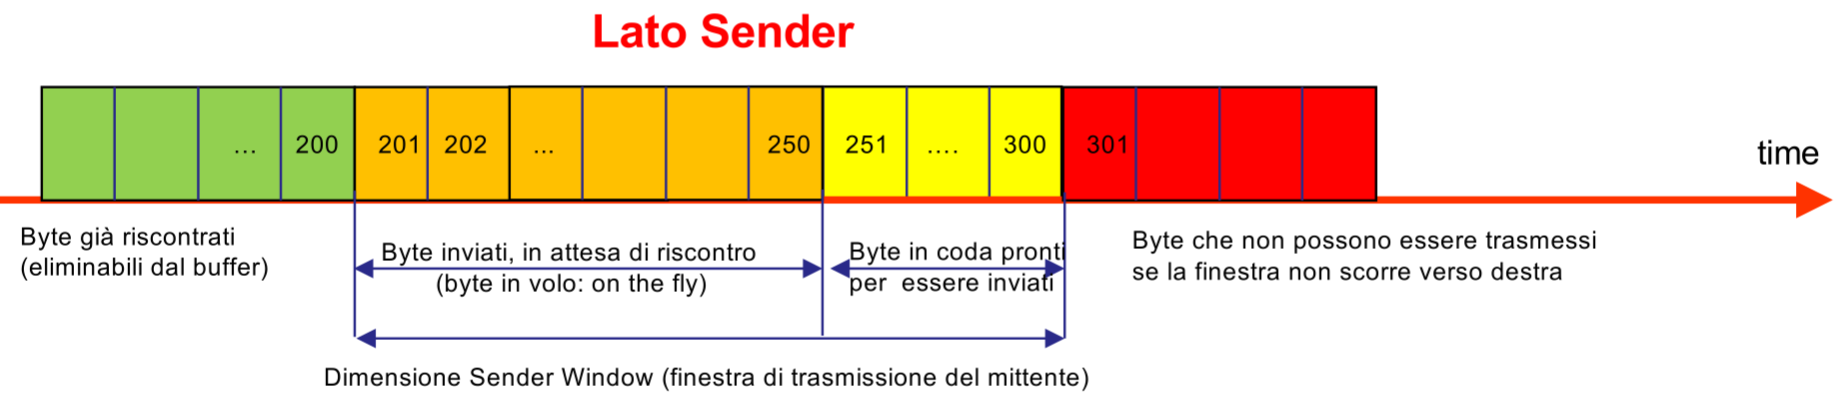
\includegraphics[width=1\textwidth]{images/finestratrasmissione.png}
    \caption{Esempio di finestra di trasmissione}
    \label{fig:finestratrasmissione}
\end{figure}

Sono gli ACK ricevuti che fanno scorrere la finestra. Se ricevo l'ACK 240 allora la finestra scorre fino a 240(riscontri cumulativi, non devo dicevere quelli 201, 202 ecc..., ma mi basta 240 per scorrere anche tutti i byte precedenti a 240).




\begin{figure}[h!]
    \centering
    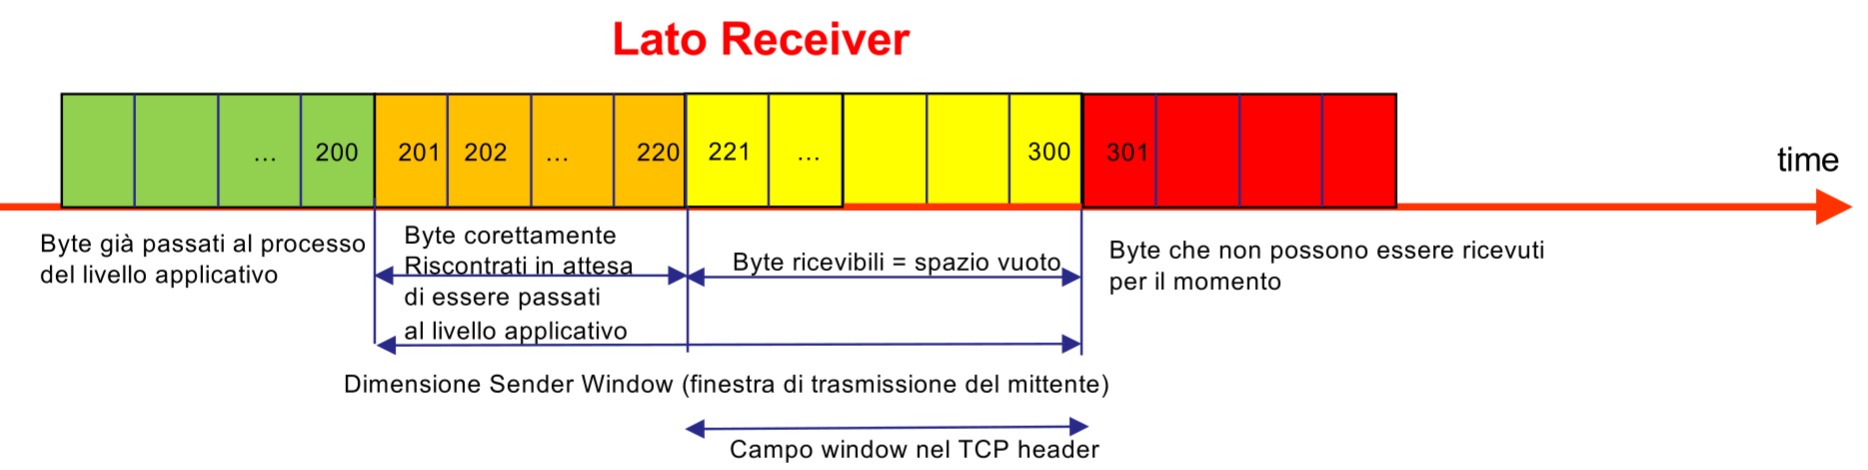
\includegraphics[width=1\textwidth]{images/finestraricezione.png}
    \caption{Esempio di finestra di ricezione}
    \label{fig:finestraricezione}
\end{figure}



\subsection{Controllo di flusso - come gestisce il TCP il flusso dei dati?}

\begin{figure}[h!]
    \centering
    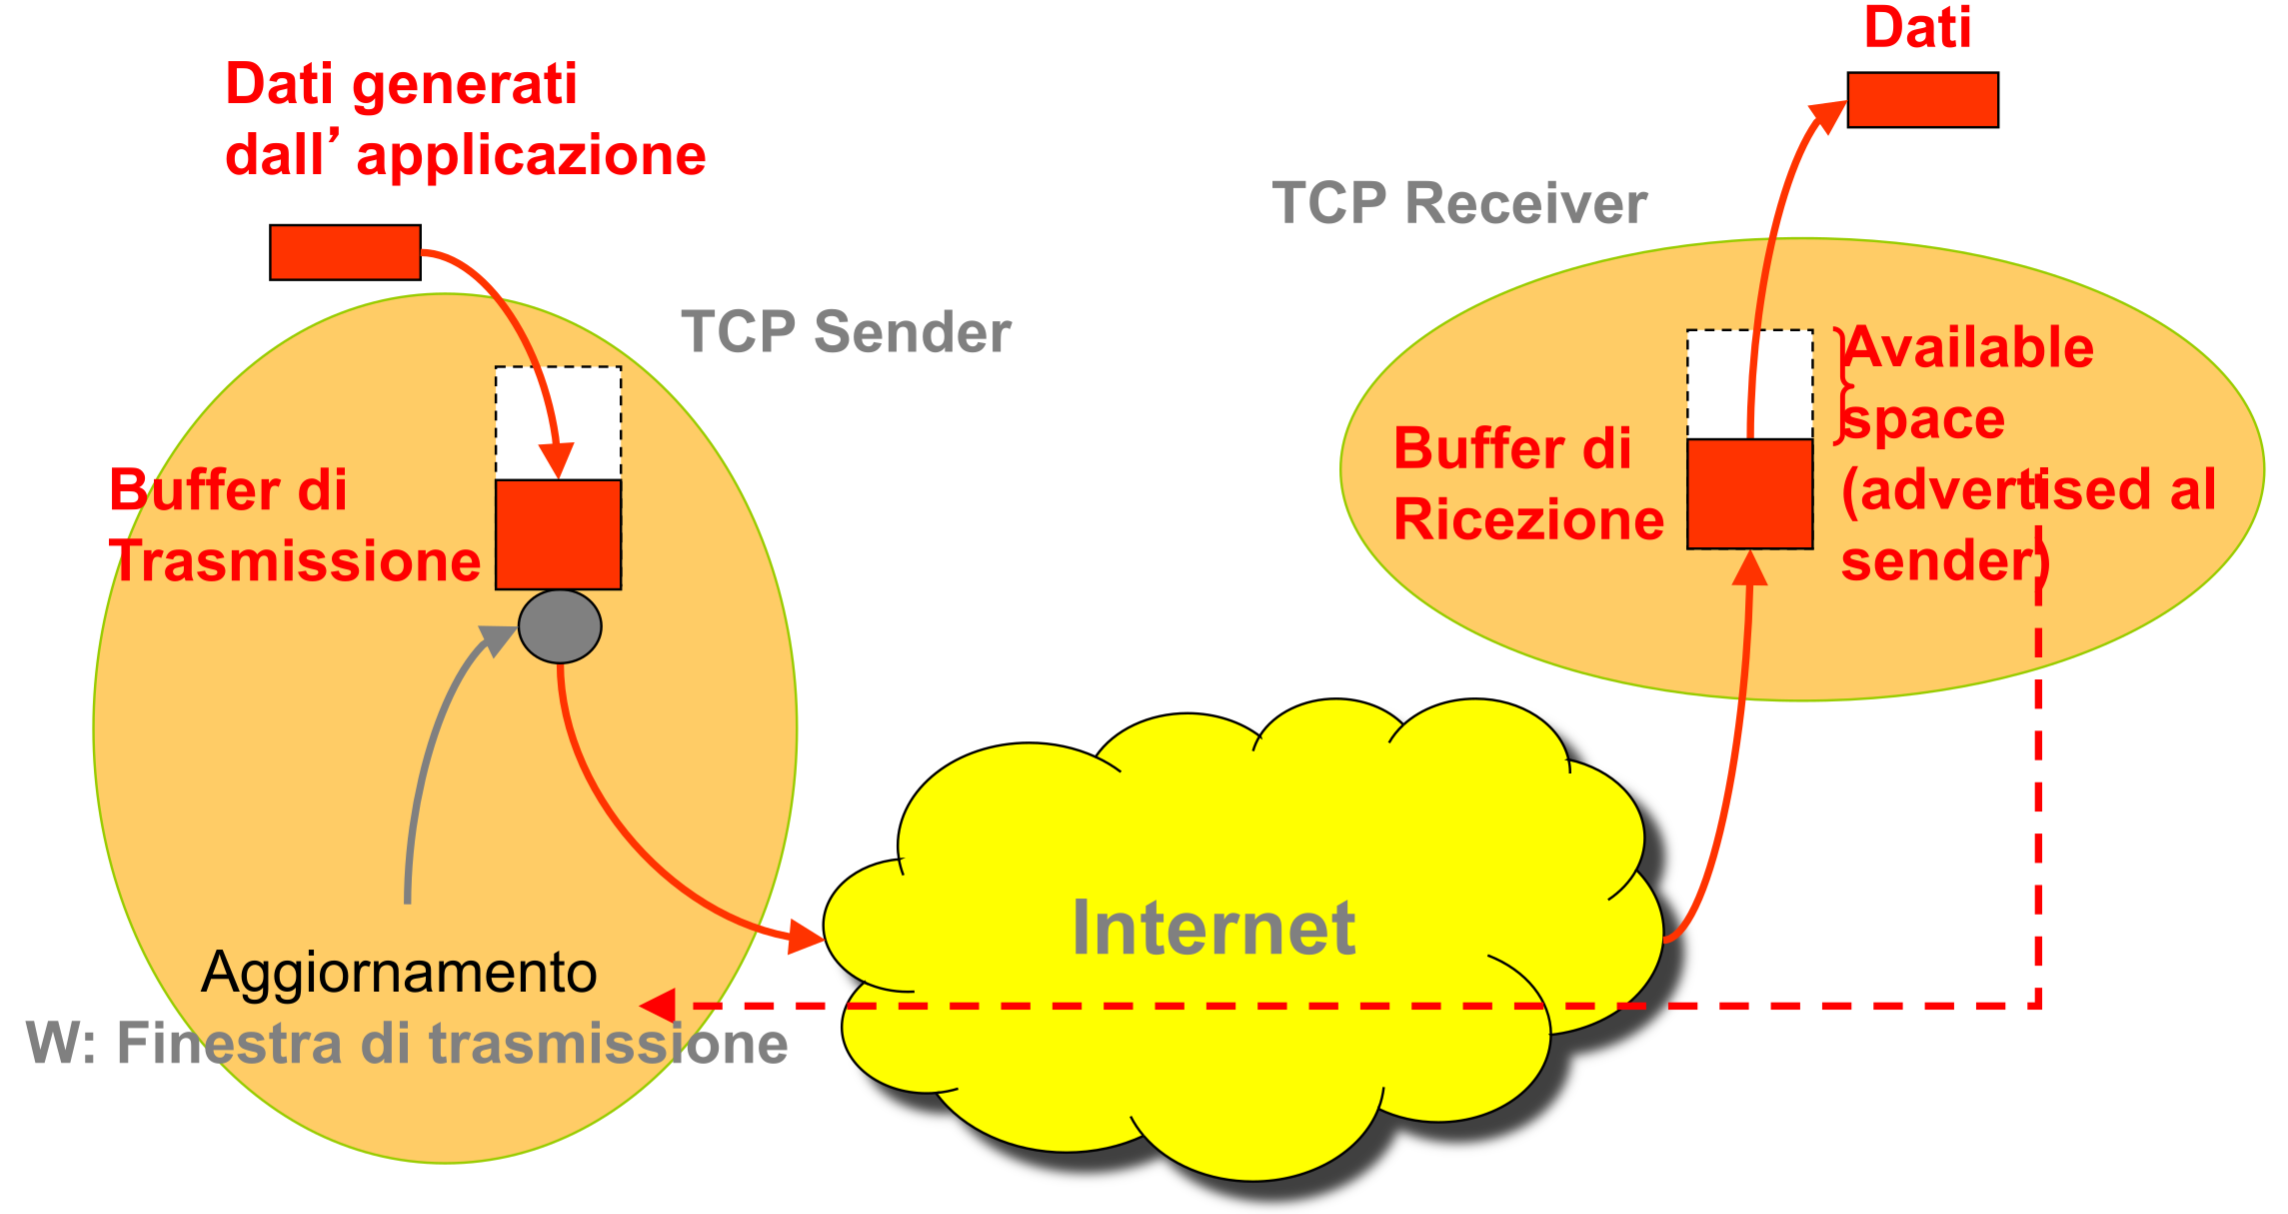
\includegraphics[width=0.8\textwidth]{images/tcpflusso.png}
    \caption{Esempio di flusso TCP}
    \label{fig:tcpflusso}
\end{figure}


IMPORTANTE: ciò che è presente nel buffer di ricezione è stato riscontrato dal mittente.

Il receiver comunica con il sender la dimensione del buffer di ricezione, in modo che il mittente possa regolare la velocità di invio dei segmenti, quindi regolare la finestra di trasmissione.


\newpage
\subsection{Perdita di segmenti - RTO e 3 dupack} 
Si assume che un segmento sia stato perso se si verificano: 3 dupack, RTO.

 \subsubsection{Retransmission Time Out - RTO}
\begin{figure}[h!]
    \centering
    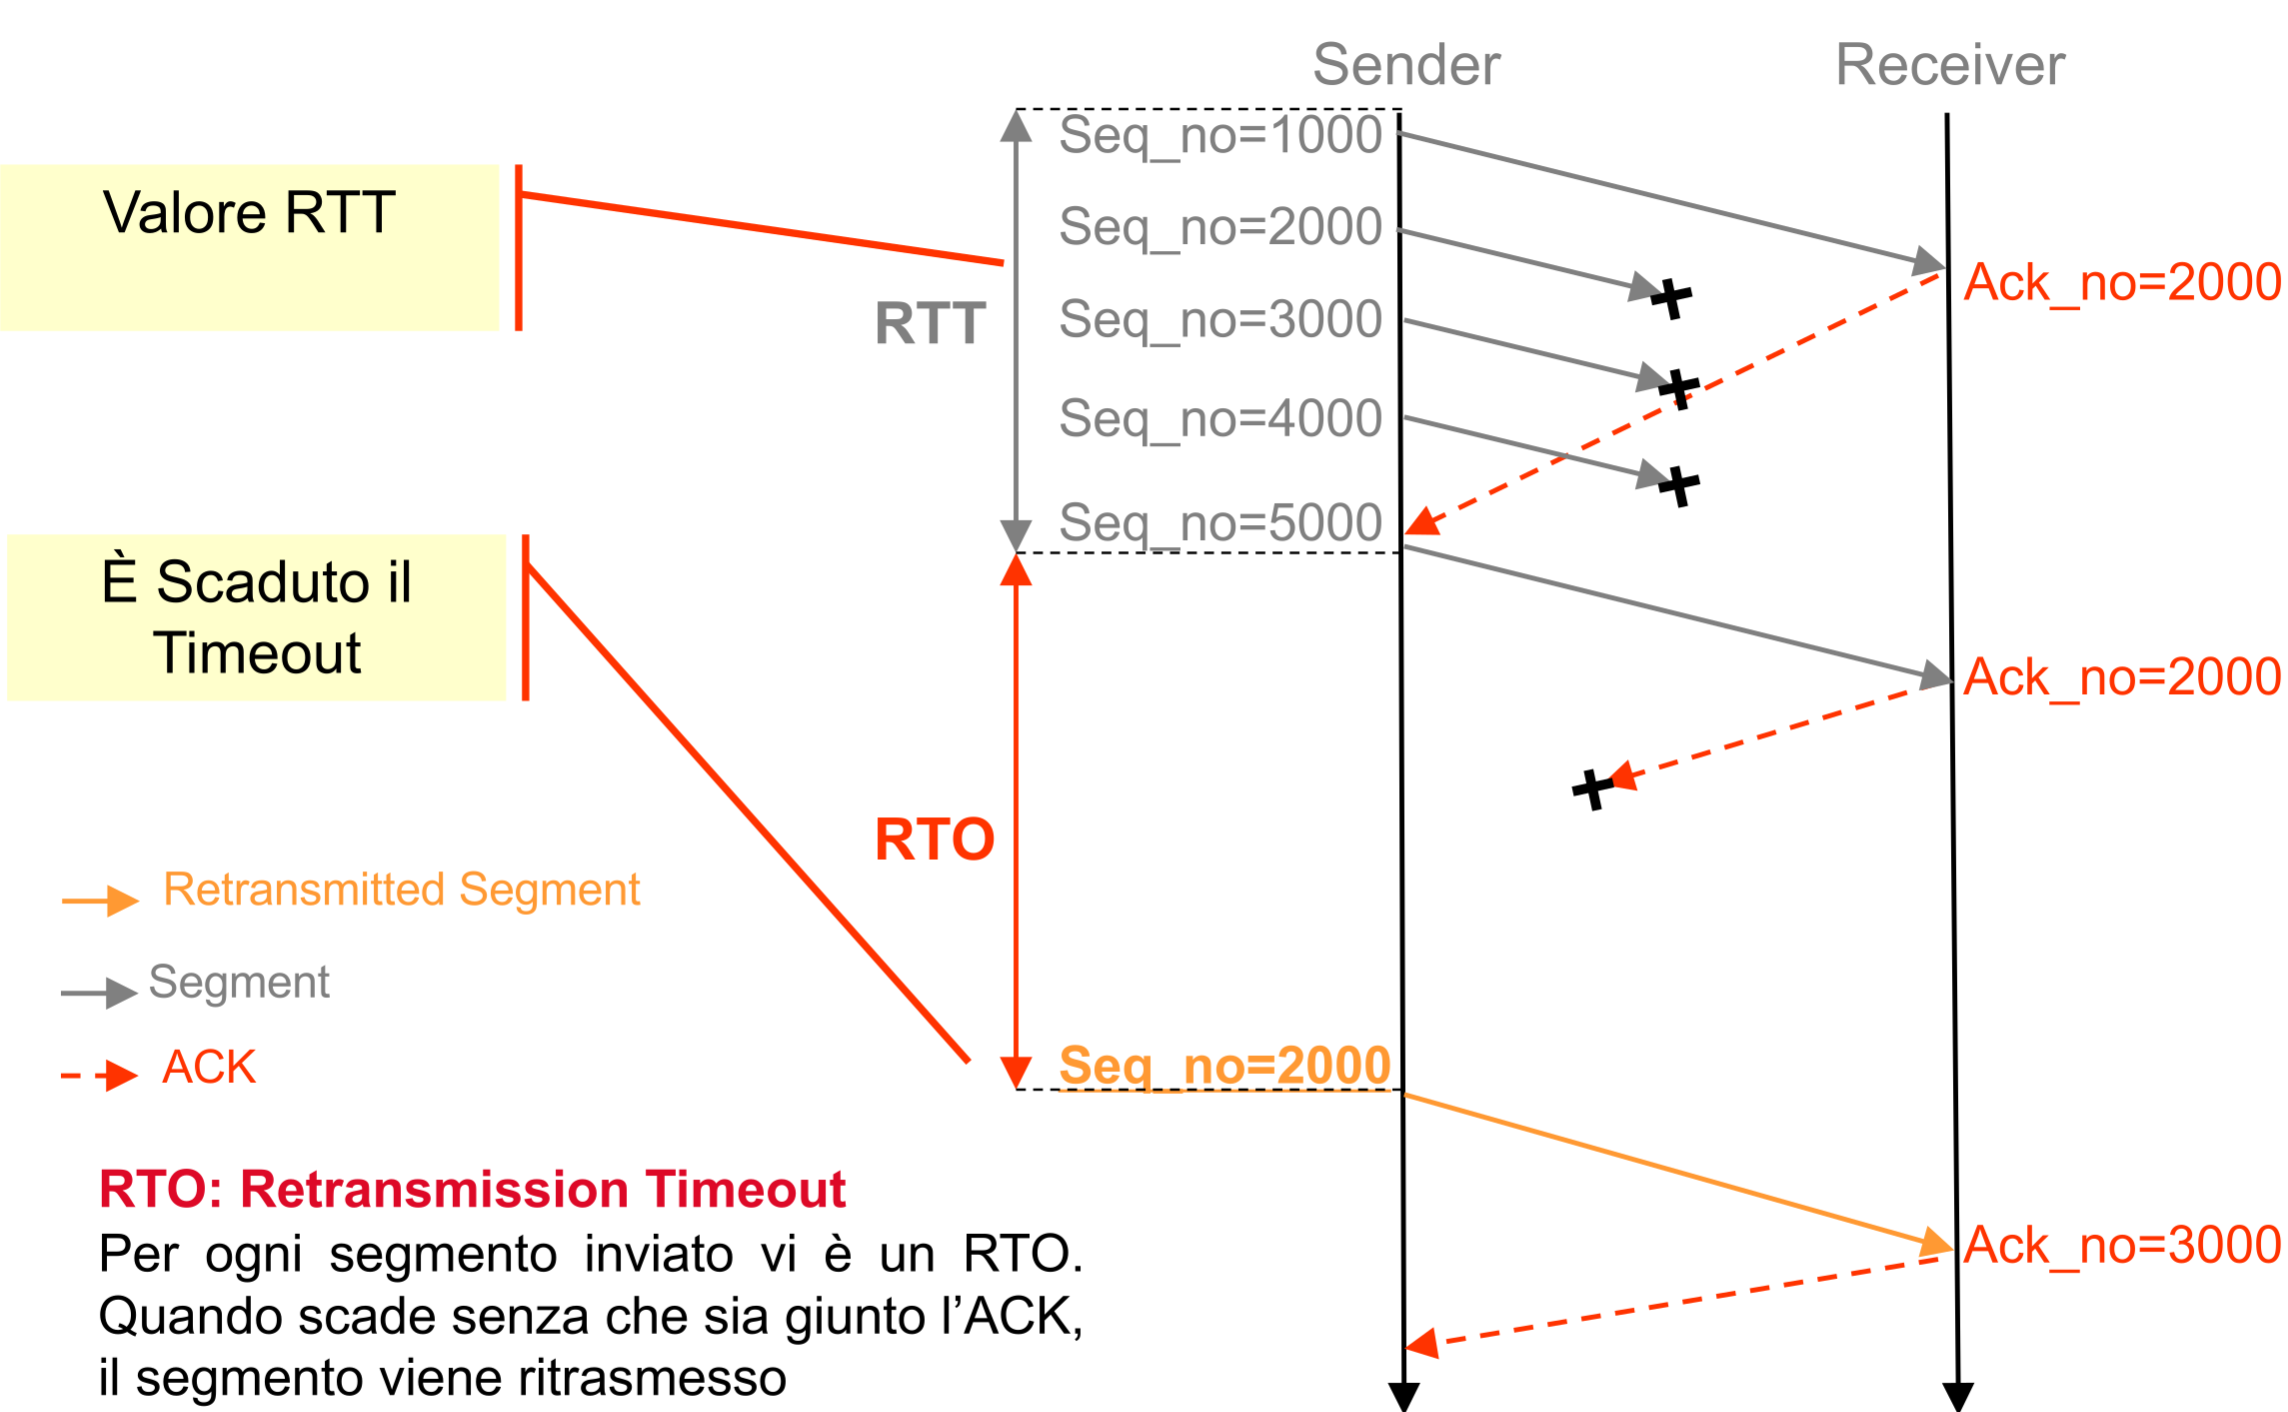
\includegraphics[width=0.9\textwidth]{images/rtotcp.png}
    \caption{Esempio di Retransmission Time Out (RTO) in TCP}
    \label{fig:rtotcp}
\end{figure}
Per ogni segmento inviato, viene avviato un RTO, ossia un timer che scade dopo un certo intervallo di tempo. Se il timer scade prima di ricevere l'ACK, il mittente ritrasmette il segmento.
\paragraph{Calcolo del RTO}

?

\newpage
\subsubsection{3 Dupack(three duplicate ACK)}
\begin{figure}[h!]
    \centering
    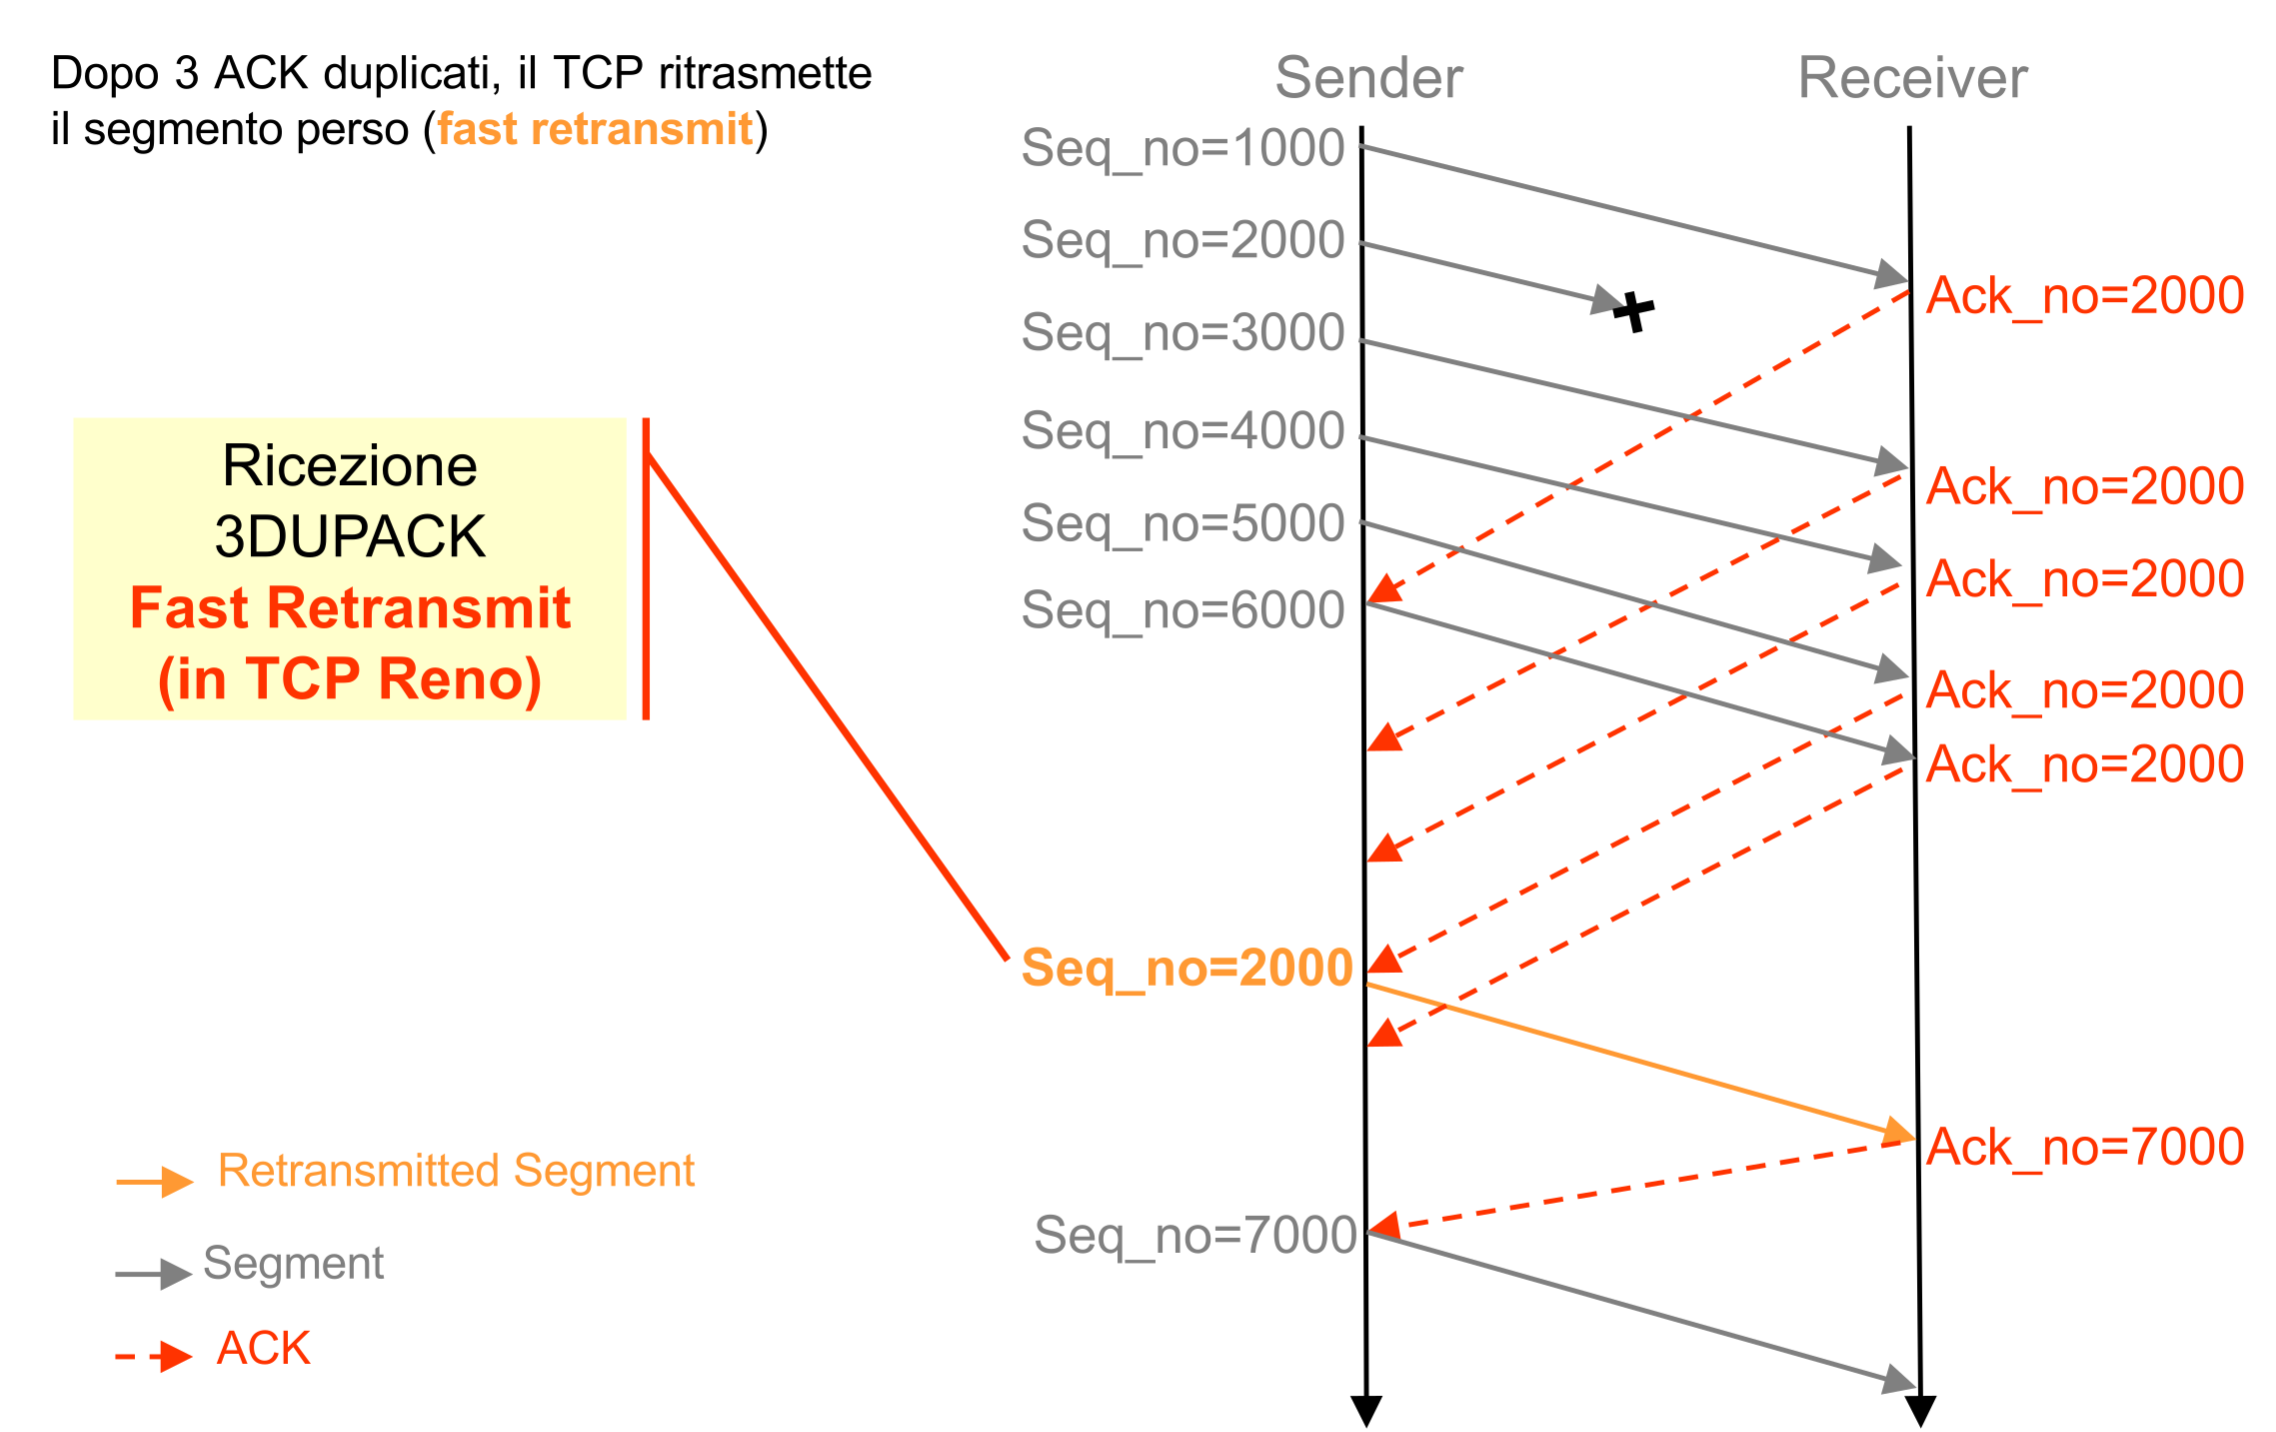
\includegraphics[width=0.8\textwidth]{images/3dupack.png}
    \caption{Esempio di 3 duplicate ACK (3 Dupack) in TCP}
    \label{fig:3dupack}
\end{figure}
\subsection{Controllo di congestione TCP}

I problemi di congestione si verificano quando la rete è sovraccarica(buff di ricezione saturo) di traffico e non riesce a gestire tutte le richieste. TCP utilizza diversi algoritmi per gestire la congestione e garantire una trasmissione affidabile dei dati.

Il protocollo TCP si rende conto dei limiti della rete solo quando avviene una congestione, quindi il TCP testa i limiti della rete(probing).

A tal scopo è importante definire le seguenti variabili:
\begin{itemize}
    \item rwnd(ricezione): è la dimensione della finestra di ricezione, ossia la quantità di dati che il mittente può inviare prima di ricevere un ACK dal destinatario.  
    \item cwnd(finestra di congestione): è dinamicamente calcolata tramite un algoritmo di controllo di congestione. 
\end{itemize}
\begin{figure}[h!]
    \begin{minipage}{0.45\textwidth}
        \centering
        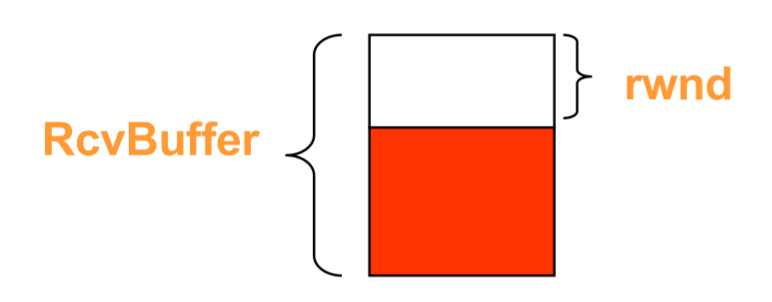
\includegraphics[width=\textwidth]{images/rwnd.png}
        \caption{Esempio di finestra di ricezione (rwnd) in TCP}
        \label{fig:rwnd}
    \end{minipage}
    \hfill
    \begin{minipage}{0.52\textwidth}
        \raggedright
        La finestra di trasmissione W è posta uguale al minimo tra la congestion window e la rwnd:
        \begin{equation}
            W = min(cwnd, rwnd)
        \end{equation}
        \raggedleft
    \end{minipage}
\end{figure}
Tramite la formula di W è possibile capire che questa finestra dipende da due variabili, una controllabile dal mittente(cwnd) ed una che dipende dal ricevente(rwnd).

La variabile cwnd ha il vantaggio di poter essere controllata, perciò se c'è una congestione in atto posso diminuire la variabile cwnd, modificando perciò la finestra di trasmissione W e la velocità di trasmissione, così da evitare di saturare la rete.

\subsubsection{Algoritmo di controllo di congestione}

\paragraph{Additive Increase Multiplicative Decrease (AIMD)}
TCP aumenta la finestra di ricezione rallentando "addittivamente" la velocità di invio dei segmenti(inzialmente è molto veloce, piano piano questa velocità tende a diminuire in modo additivo). 

Quando però avviene una congestione, la finestra non viene rallentata in modo additivo, ma anzi, viene ridotta drasticamente in modo moltiplicativo, moltiplicando la finestra per un fattore frazionario. 


\subsubsection{Evoluzione della cwnd}

        \paragraph{Slow start}
        Inizialmente la cwnd è pari ad 1 MSS, minimo valore possibile di cwnd, invia un segmento e inizia la fase di probing(slow start: parte "piano" per poi aumentare). Ogni volta che si ha un riscontro viene raddoppiata la cwnd. 

        \begin{itemize}
            \item MSS(maximum segment size): rappresenta la massima quantità di dati (in byte) che un host TCP può ricevere in un singolo segmento.
            tipicamnete 1460 byte (se MTU = 1500 e header IP+TCP = 40 byte)
            \item sstresh(slow star threshold): è una soglia che separa la fase di Slow Start da quella di Congestion Avoidance
        \end{itemize}

        Quando si verifica una congestione(3DUPACK o scadenza RTO), la cwnd e la soglia sshtresh(viene posta pari alla metà della finestra di congestione al momento della congestione) vengono modificate in base all'algoritmo di congestione utilizzato.

        \paragraph{Congestion avoidance}
        Nel caso in cui  la cwnd sia maggiore della soglia sshtresh, inizia la fase di congestion avoidance, in cui la cwnd viene aumentata linearmente, ossia viene incrementata di 1 MSS ogni RTT.

        L'obiettivo è quello di aumentare la cwnd in modo più lento, evitando di saturare la rete.
        \begin{equation}
            cwnd = cwnd + \frac{1}{\text{cwnd}}     \end{equation}
        
  
        \begin{figure}[h!]
        \centering
        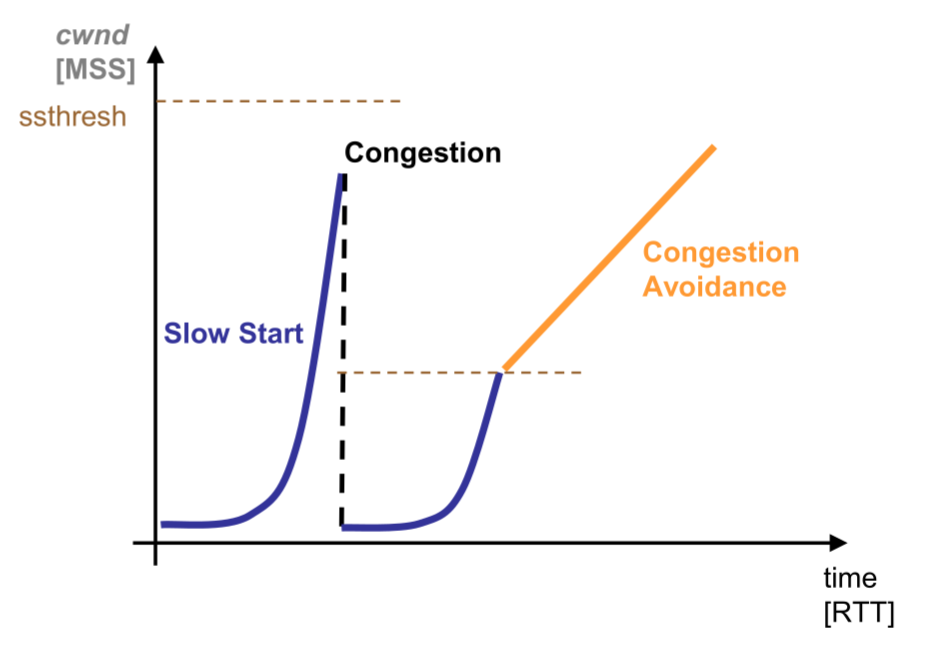
\includegraphics[width=0.75\textwidth]{images/graficocongestione.png}
        \caption{Andamento della finestra di congestione}
        \label{fig:graficocongestione}
        \end{figure}

        \newpage

\subsubsection{TCP Tahoe}

\begin{figure}[h!]
    \begin{minipage}{0.6\textwidth}
        \centering
        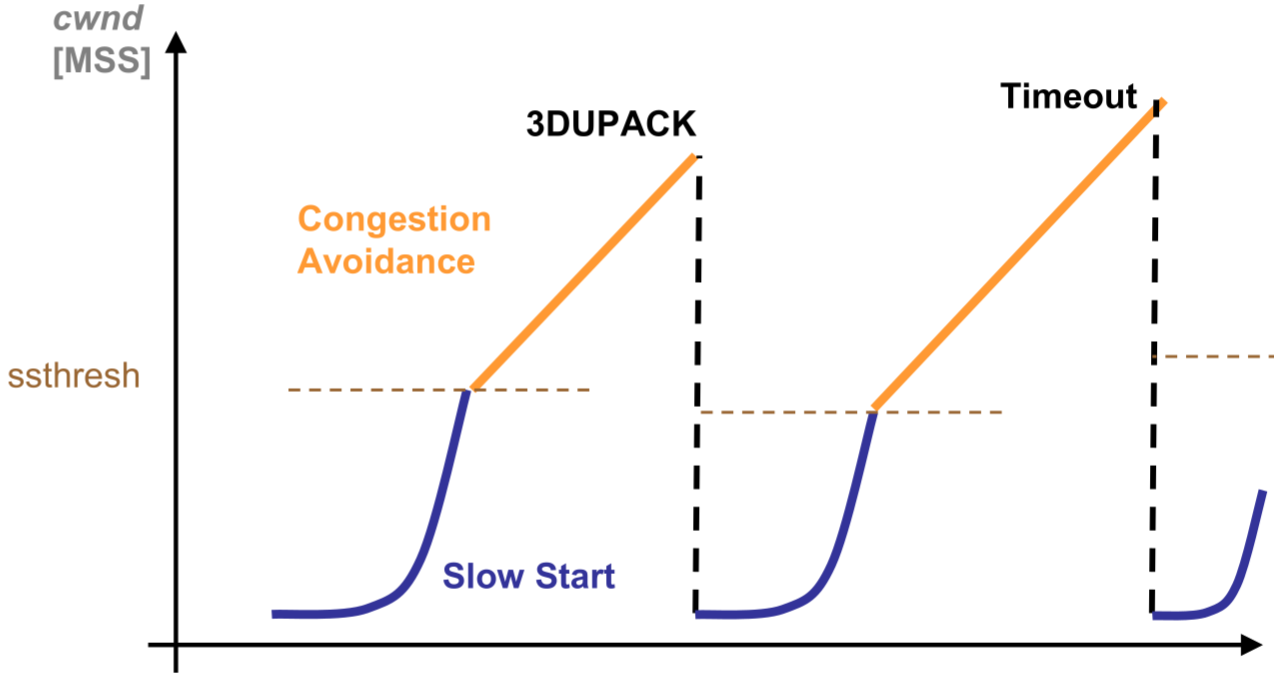
\includegraphics[width=0.95\textwidth]{images/tahoe.png}
        \caption{Andamento della finestra di congestione in Tahoe}
        \label{fig:tcptahoe}
    \end{minipage}
    \hfill
    \begin{minipage}{0.48\textwidth}
        TCP Tahoe non distingue tra i due eventi di congestione(3DUPACK e RTO), quando avviene riporta la cwnd a 1; rientrando in slow start.
    \end{minipage}
\end{figure}

\subsubsection{TCP Reno}

\begin{figure}[h!]
    \begin{minipage}{0.6\textwidth}
        \centering
        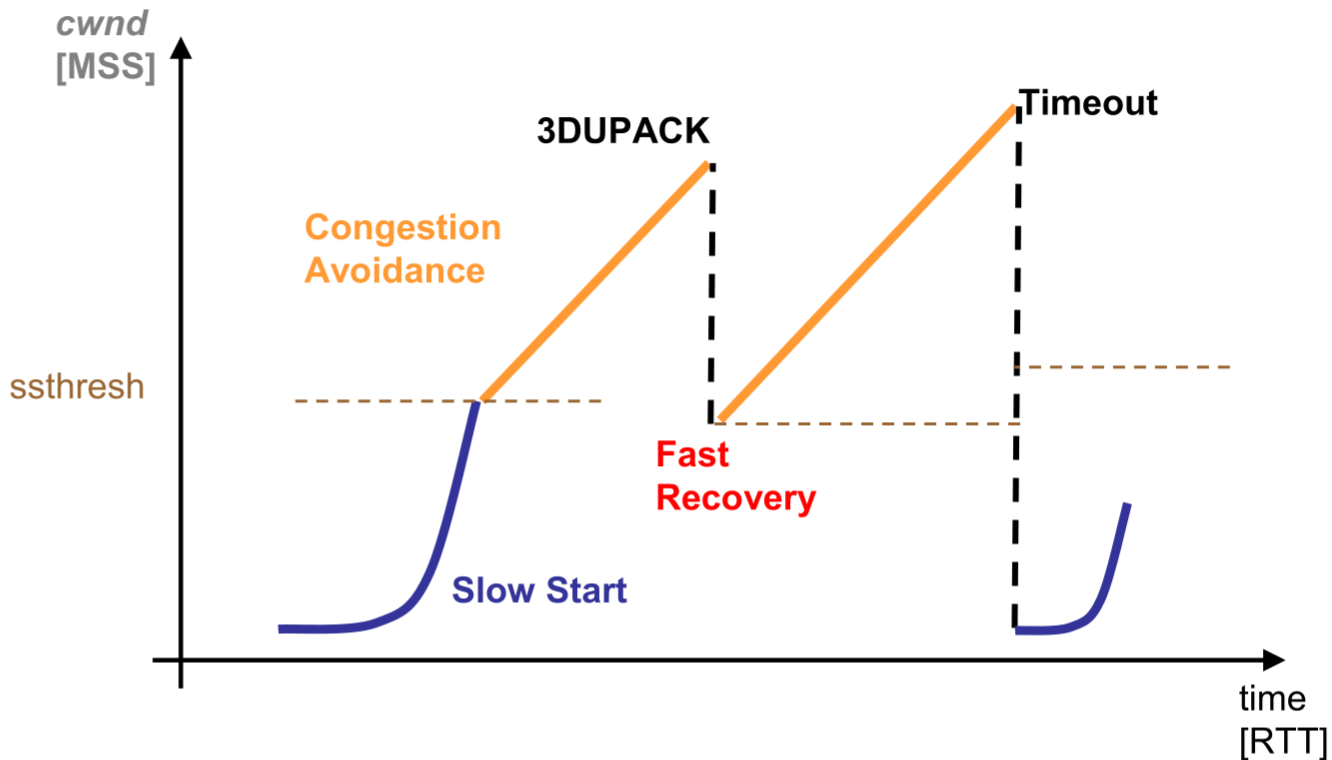
\includegraphics[width=0.95\textwidth]{images/reno.png}
        \caption{Andamento della finestra di congestione in Reno}
        \label{fig:tcpreno}
    \end{minipage}
    \hfill
    \begin{minipage}{0.48\textwidth}
        TCP Reno distingue i due eventi di congestione, (considerando che un 3DUPACK è un evento di congestione più "leggero" rispetto ad un RTO):
            \begin{itemize}
                \item In caso di 3DUPACK, la cwnd viene dimezzata e si entra nella fase di fast recovery, in cui la cwnd viene aumentata linearmente fino a raggiungere la soglia sshtresh.
                \item In caso di RTO, la cwnd viene riportata a 1 e si entra nella fase di slow start.
            \end{itemize}   
    \end{minipage}
\end{figure}

\subsubsection{TCP New Reno}

\begin{figure}[h!]
    \begin{minipage}{0.6\textwidth}
        \centering
        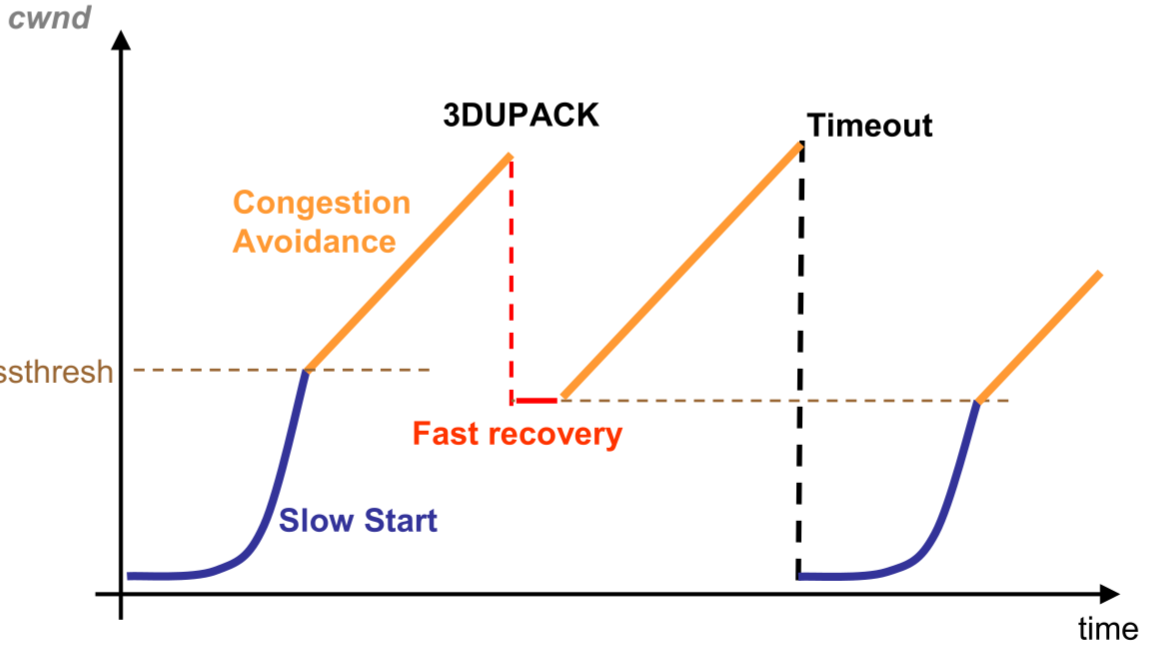
\includegraphics[width=0.95\textwidth]{images/newreno.png}
        \caption{Andamento della finestra di cong. in New Reno}
        \label{fig:tcpnewreno}
    \end{minipage}
    \hfill
    \begin{minipage}{0.48\textwidth}
        Nel reno visto in precedenza ad ogni 3DUPACK viene dimezzata la cwnd, ma questo non è ottimale nel caso in cui avvengano più 3DUPACK nella stessa finestra.

        Perciò esiste la variante New Reno, che non dimezza la cwnd ad ogni 3DUPACK, lo fa solamente la prima volta che avviene all'interno della finestra; quelli successivi vengono ignorati.
    \end{minipage}
\end{figure}